% -*- mode: tex; fill-column: 115; -*-

%\documentclass[twoside]{article}
\usepackage[top=1in, left=0.5in, right=0.5in, bottom=0.3in,paperheight=8.5in,paperwidth=5.5in]{geometry}
\setcounter{secnumdepth}{5}
\setcounter{tocdepth}{5}
\usepackage[english]{babel}
\usepackage{textcomp}
\usepackage[fit]{truncate}
\usepackage{fancyhdr}
\pagestyle{fancy}
\renewcommand{\sectionmark}[1]{\markboth{#1}{}}
\fancyhead{}
\fancyhead[OR]{\leftmark \hspace{0.1cm}  $\vert$ \hspace{0.1cm}  \thepage}
\fancyhead[EL]{\thepage \hspace{0.1cm} $\vert$ \hspace{0.1cm} \leftmark}
\fancyfoot[C]{}%hide footer
\usepackage[hidelinks,plainpages=false]{hyperref}
\usepackage{bibentry}

\usepackage{amsmath,amsthm,amsfonts,amssymb,epsfig}
\usepackage{array}
\usepackage{datetime}
\usepackage{lipsum}% http://ctan.org/pkg/lipsum
\usepackage{listings}% http://ctan.org/pkg/listings
\usepackage{spverbatim}
\usepackage{hyperref}
\usepackage{xcolor} 
\usepackage[scaled=1]{couriers}
\xdefinecolor{gray}{rgb}{0.6,0.6,0.6} 
\Urlmuskip=0mu plus 1mu\relax %needed to make long URLs break nicely
\usepackage{microtype}
\definecolor{links}{HTML}{2A1B81}
\hypersetup{colorlinks,linkcolor=,urlcolor=links,citecolor=links}
\usepackage{graphicx}
\graphicspath{ {images/} }
\usepackage{parskip}
\usepackage{titlesec} %used for diminishing heading sizes
\titleformat{\section}{\normalfont\bfseries}{\thesection}{1em}{}
\titlespacing*{\section}{0pt}{*2}{0pt}
\titlespacing*{\subsection}{0pt}{*2}{0pt}
\usepackage[square, sort, comma, numbers]{natbib} %%uses titles for cited references
\usepackage[fit]{truncate}
\usepackage{fancyhdr}
\pagestyle{fancy}
\renewcommand{\sectionmark}[1]{\markboth{#1}{}}
\fancyhead{}
\fancyhead[OR]{\leftmark \hspace{0.1cm}  $\vert$ \hspace{0.1cm}  \thepage}
\fancyhead[EL]{\thepage \hspace{0.1cm} $\vert$ \hspace{0.1cm} \leftmark}
\fancyfoot[C]{}%hide footer 
\usepackage{setspace}
\usepackage{adjustbox} 
\usepackage[all]{nowidow} %prevent widows/orphans
\usepackage{bibentry}
\usepackage{standalone}

\documentclass[twoside]{article}
\usepackage[top=1in, left=0.5in, right=0.5in, bottom=0.5in,paperheight=8.5in,paperwidth=5.5in]{geometry}
\setcounter{secnumdepth}{5}
\setcounter{tocdepth}{5}
\usepackage[english]{babel}
\usepackage{textcomp}
\usepackage[fit]{truncate}
\usepackage{fancyhdr}
\pagestyle{fancy}
\renewcommand{\sectionmark}[1]{\markboth{#1}{}}
\fancyhead{}
\fancyhead[OR]{\leftmark \hspace{0.1cm}  $\vert$ \hspace{0.1cm}  \thepage}
\fancyhead[EL]{\thepage \hspace{0.1cm} $\vert$ \hspace{0.1cm} \leftmark}
\fancyfoot[C]{}%hide footer
\usepackage[hidelinks,plainpages=false]{hyperref}
\usepackage{bibentry}
\usepackage{amsmath,amsthm,amsfonts,amssymb,epsfig}
\usepackage{array}
\usepackage{datetime}
\usepackage{lipsum}% http://ctan.org/pkg/lipsum
\usepackage{listings}% http://ctan.org/pkg/listings
\usepackage{spverbatim}
\usepackage{hyperref}
\usepackage{xcolor} 
\usepackage[scaled=1]{couriers}
\xdefinecolor{gray}{rgb}{0.6,0.6,0.6} 
\Urlmuskip=0mu plus 1mu\relax %needed to make long URLs break nicely
\usepackage{microtype}
\hypersetup{colorlinks=false}
\usepackage{graphicx}
\graphicspath{ {images/} }
\usepackage{parskip}
\usepackage{titlesec} %used for diminishing heading sizes
\titleformat{\section}{\normalfont\bfseries}{\thesection}{1em}{}
\titlespacing*{\section}{0pt}{*2}{0pt}
\titlespacing*{\subsection}{0pt}{*2}{0pt}
\usepackage[square, sort, comma, numbers]{natbib} %%uses titles for cited references

%\usepackage[square,authoryear,sort&compress]{natbib}
%[square, sort, comma, numbers]{natbib} %%uses titles for cited references

\usepackage{xcolor} 
\usepackage[scaled=1]{couriers}
\usepackage{graphicx}
\xdefinecolor{gray}{rgb}{0.6,0.6,0.6} 
\usepackage{setspace}
\usepackage{adjustbox} 
\usepackage[all]{nowidow} %prevent widows/orphans [all,defaultlines]
\usepackage{standalone}

  %settings for printed booklets - comment out by default, uncomment for print and comment out line above. don't save this change! "conf_top" should be default

\defcitealias{glmnet}{Regularization Paths for Generalized Linear Models via Coordinate Descent by Friedman et. al}

\defcitealias{strongrules}{Strong Rules for Discarding Predictors in Lasso-type Problems by Bien et. al}

\defcitealias{admm}{Distributed Optimization and Statistical Learning via the Alternating Direction Method of Multipliers by Boyd et. al}

\defcitealias{prox}{Proximal Algorithms by Boyd et. al}


\titleformat*{\section}{\LARGE\bfseries\sffamily}
\titleformat*{\subsection}{\Large\bfseries\sffamily}
\titleformat*{\subsubsection}{\large\bfseries\sffamily}
\titleformat*{\paragraph}{\large\bfseries\sffamily}
\titleformat*{\subparagraph}{\large\bfseries\sffamily}
\renewcommand{\familydefault}{\sfdefault} %sans-serif font



%----------------------------------------------------------------------
% Definition for "lstlisting" blocks
%----------------------------------------------------------------------
% --- USAGE ---
%
% \begin{lstlisting}[style=R}
% ...
% \end{lstlisting}
%
% % \begin{lstlisting}[style=output}
% ...
% \end{lstlisting}
%----------------------------------------------------------------------

% By default, make listings all black so it's easy to spot the ones that aren't set to a style.
% This is just a debugging technique.
\lstset{backgroundcolor=\color{black}}

% Define scala language first
% ``define'' Scala
\lstdefinelanguage{scala}{
  morekeywords={abstract,case,catch,class,def,%
    do,else,extends,false,final,finally,%
    for,if,implicit,import,match,mixin,%
    new,null,object,override,package,%
    private,protected,requires,return,sealed,%
    super,this,throw,trait,true,try,%
    type,val,var,while,with,yield},
  otherkeywords={=>,<-,<\%,<:,>:,\#,@},
  sensitive=true,
  morecomment=[l]{//},
  morecomment=[n]{/*}{*/},
  morestring=[b]``,
  morestring=[b]',
  morestring=[b]''``
}

\lstdefinestyle{R}{
  language=R,
  frame=single,
  breaklines,
  basicstyle=\ttfamily,
  commentstyle=\textbf,% comment style
  keywordstyle=\ttfamily,
  numbers=left,% display line numbers on the left side 
  numberstyle=\scriptsize,% use small line numbers 
  numbersep=10pt,% space between line numbers and code
  backgroundcolor=\color{white}, 
  showstringspaces=false % don't show spaces as weird char.
}

\lstdefinestyle{python}{
  language=python,
  frame=single,
  breaklines,
  basicstyle=\ttfamily,
  commentstyle=\textsl,% comment style
  keywordstyle=\ttfamily,
  numbers=left,% display line numbers on the left side 
  numberstyle=\scriptsize,% use small line numbers 
  numbersep=10pt,% space between line numbers and code
  backgroundcolor=\color{white}, 
  showstringspaces=false %don't show spaces as weird char.
}

\lstdefinestyle{Scala}{
  language=scala,
  frame=single,
  breaklines,
  basicstyle=\ttfamily,
  commentstyle=\textsl,% comment style
  keywordstyle=\ttfamily,
  numbers=left,% display line numbers on the left side 
  numberstyle=\scriptsize,% use small line numbers 
  numbersep=10pt,% space between line numbers and code
  backgroundcolor=\color{white}, 
  showstringspaces=false % don't show spaces as weird char.
}

\lstdefinestyle{Bash}{
  language=bash,
  frame=single,
  breaklines,
  basicstyle=\ttfamily,
  commentstyle=\textsl,% comment style
  keywordstyle=\ttfamily,
  numbers=left,% display line numbers on the left side 
  numberstyle=\scriptsize,% use small line numbers 
  numbersep=10pt,% space between line numbers and code
  backgroundcolor=\color{white}, 
  showstringspaces=false % don't show spaces as weird char.
}


\definecolor{mygray}{rgb}{0.92,0.92,0.92}

\lstdefinestyle{output}{
  frame=single,
  breaklines,
  basicstyle=\ttfamily,
  numbers=left,% display line numbers on the left side 
  numberstyle=\scriptsize,% use small line numbers 
  numbersep=10pt,% space between line numbers and code
  backgroundcolor=\color{mygray}, 
  showstringspaces=false %don't show spaces as weird char.
}

\newcommand{\waterExampleInR} {
\textbf{Example in R} \\
}

\newcommand{\waterExampleInPython} {
\textbf{Example in Python} \\
}
 %see note for `conf_top_print.tex` above
%% TO DO: Find better templates for R and Python



%----------------------------------------------------------------------
% Definition for "lstlisting" blocks
%----------------------------------------------------------------------
% --- USAGE ---
%
% \begin{lstlisting}[style=R}
% ...
% \end{lstlisting}
%
% % \begin{lstlisting}[style=output}
% ...
% \end{lstlisting}
%----------------------------------------------------------------------

% By default, make listings all black so it's easy to spot the ones that aren't set to a style.
% This is just a debugging technique.
%\lstset{backgroundcolor=\color{black}}

% http://latexcolor.com/
\definecolor{deepblue}{rgb}{0,0,0.5}
\definecolor{deepred}{rgb}{0.6,0,0}
\definecolor{deepgreen}{rgb}{0,0.5,0}
%\definecolor{tan}{rgb}{0.98, 0.92, 0.84}  %antiquewhite
%\definecolor{r_bkgd}{rgb}{1.0, 0.92, 0.8}  %blacnedalmond
\definecolor{py_bkgd}{rgb}{0.94, 0.97, 1.0}  %aliceblue
\definecolor{ashgrey}{rgb}{0.7, 0.75, 0.71}
\definecolor{battleshipgrey}{rgb}{0.52, 0.52, 0.51}
%\definecolor{r_bkgd}{rgb}{0.97, 0.91, 0.81}  %champagne
\definecolor{r_bkgd}{rgb}{0.98, 0.92, 0.84}  %moccasin

\definecolor{Code}{rgb}{0,0,0}
\definecolor{Decorators}{rgb}{0.5,0.5,0.5}
\definecolor{Numbers}{rgb}{0.5,0,0}
\definecolor{MatchingBrackets}{rgb}{0.25,0.5,0.5}
\definecolor{Keywords}{rgb}{0,0,1}
\definecolor{self}{rgb}{0,0,0}
\definecolor{Strings}{rgb}{0,0.63,0}
\definecolor{Comments}{rgb}{0,0.63,1}
\definecolor{Backquotes}{rgb}{0,0,0}
\definecolor{Classname}{rgb}{0,0,0}
\definecolor{FunctionName}{rgb}{0,0,0}
\definecolor{Operators}{rgb}{0,0,0}
\definecolor{Background}{rgb}{0.98,0.98,0.98}

% KEYWORDS
% http://tex.stackexchange.com/questions/186092/how-can-i-delete-non-letter-keywords-such-as
\lstdefinestyle{Scala}{
  language={Scala},
  frame=single,
  breaklines,
  basicstyle=\ttfamily,
  commentstyle=\itshape\color{battleshipgrey},% comment style
  %commentstyle=\textsl,% comment style
  %keywordstyle=\ttfamily\color{deepblue},
  %keywordstyle=\color{WildStrawberry},
  numbers=left,% display line numbers on the left side
  numberstyle=\scriptsize,% use small line numbers
  numbersep=10pt,% space between line numbers and code
  backgroundcolor=\color{white},
  showstringspaces=false,
  stringstyle=\color{deepgreen},
  backgroundcolor=\color{py_bkgd},
  % keywords
  morekeywords={abstract,case,catch,class,def,%
    do,else,extends,false,final,finally,%
    for,if,implicit,import,match,mixin,%
    new,null,object,override,package,%
    private,protected,requires,return,sealed,%
    super,this,throw,trait,true,try,%
    type,val,var,while,with,yield},
  otherkeywords={=>,<-,<\%,<:,>:,\#,@},
  sensitive=true,
  morecomment=[l]{//},
  morecomment=[n]{/*}{*/},
  morestring=[b]``,
  morestring=[b]',
  morestring=[b]''``,
  keywordstyle={\color{Keywords}\bfseries},
}

\lstdefinestyle{R}{
  language={R},
  frame=single,
  breaklines,
  basicstyle=\ttfamily,
  %commentstyle=\textsl\color{Comments},% comment style
  commentstyle=\itshape\color{battleshipgrey},% comment style
  keywordstyle=\ttfamily\color{deepblue},
  numbers=left,% display line numbers on the left side 
  numberstyle=\scriptsize,% use small line numbers 
  numbersep=10pt,% space between line numbers and code
  backgroundcolor=\color{r_bkgd},
  showstringspaces=false,
  stringstyle=\color{deepgreen},
  %morekeywords={TRUE, FALSE, for, if},
  keywordstyle={\color{Keywords}\bfseries},
  keywords={TRUE, FALSE},
  deletekeywords={grid, frame, variable, model, vi, predict, file},
  otherkeywords={!,!=,~,$,*,\&,\%/\%,\%*\%,\%\%,<-,<<-},
  %morekeywords={TRUE, FALSE, list, c}
}



\lstdefinestyle{python}{
  language={Python},
  frame=single,
  breaklines,
  basicstyle=\ttfamily,
  commentstyle=\itshape\color{battleshipgrey},% comment style
  %commentstyle=\textsl,% comment style
  %keywordstyle=\ttfamily\color{deepblue},
  %keywordstyle=\color{WildStrawberry},
  numbers=left,% display line numbers on the left side 
  numberstyle=\scriptsize,% use small line numbers 
  numbersep=10pt,% space between line numbers and code
  backgroundcolor=\color{white},
  showstringspaces=false,
  stringstyle=\color{deepgreen},
  backgroundcolor=\color{py_bkgd},
  % keywords
morekeywords={import,from,class,def,for,while,if,is,in,elif,else,not,and,or,print,break,continue,return,True,False,None,access,as,,del,except,exec,finally,global,import,lambda,pass,print,raise,try,assert},
 keywordstyle={\color{Keywords}\bfseries},
}

\lstdefinestyle{Bash}{
  language=bash,
  frame=single,
  breaklines,
  basicstyle=\ttfamily,
  commentstyle=\textsl,% comment style
  keywordstyle=\ttfamily,
  numbers=left,% display line numbers on the left side
  numberstyle=\scriptsize,% use small line numbers
  numbersep=10pt,% space between line numbers and code
  backgroundcolor=\color{white},
  showstringspaces=false % don't show spaces as weird char.
}

\definecolor{mygray}{rgb}{0.92,0.92,0.92}

\lstdefinestyle{output}{
  frame=single,
  breaklines,
  basicstyle=\ttfamily,
  numbers=left,% display line numbers on the left side 
  numberstyle=\scriptsize,% use small line numbers 
  numbersep=10pt,% space between line numbers and code
  backgroundcolor=\color{mygray},
  showstringspaces=false 
}

\newcommand{\waterExampleInR} {
\textbf{Example in R} \\
}

\newcommand{\waterExampleInPython} {
\textbf{Example in Python} \\
}
  % Work in progress....  Use this for online/pdf version

\usepackage{url}
\def\UrlBreaks{\do\/\do-\do_}

\begin{document}


\thispagestyle{empty} %removes page number
\newgeometry{bmargin=0cm, hmargin=0cm}


\begin{center}
\textsc{\Large\bf{Generalized Linear Modeling with H2O}}
\\
\small
\bigskip
\line(1,0){250}  %inserts  horizontal line 

\textsc{\small{Tomas Nykodym \hspace{10pt} Tom Kraljevic \hspace{10pt} Amy Wang \hspace{10pt} Wendy Wong}}

\textsc{\small{Edited by: Angela Bartz}}
\\
\bigskip
\line(1,0){250}  %inserts  horizontal line


{\url{http://h2o.ai/resources/}}

\bigskip
\monthname \hspace{1pt}  \the\year: Seventh Edition

 
\bigskip
\end{center}

% commenting out lines image due to print issues, but leaving for future ref. 
%\null\vfill
%\begin{figure}[!b]
%\noindent\makebox[\textwidth]{%
%\centerline{
\includegraphics[width=\paperwidth]{waves.png}}}
%\end{figure}

\newpage
\restoregeometry

\null\vfill %move next text block to lower left of new page

\thispagestyle{empty}%remove pg#


{\raggedright\vfill\ 

Generalized Linear Modeling with H2O\\

by Tomas Nykodym, Tom Kraljevic, Amy Wang \&\ Wendy Wong \\ 
with assistance from Nadine Hussami \&\ Ariel Rao \\
Edited by: Angela Bartz

\bigskip
  Published by H2O.ai, Inc. \\
2307 Leghorn St. \\
Mountain View, CA 94043\\
\bigskip
\textcopyright 2016-\the\year \hspace{1pt} H2O.ai, Inc. All Rights Reserved. 
\bigskip

\monthname \hspace{1pt}  \the\year: Sixth Edition
\bigskip

Photos by \textcopyright H2O.ai, Inc.
\bigskip

All copyrights belong to their respective owners.\\
While every precaution has been taken in the\\
preparation of this book, the publisher and\\
authors assume no responsibility for errors or\\
omissions, or for damages resulting from the\\
use of the information contained herein.\\
\bigskip
Printed in the United States of America. 
}

\newpage
\thispagestyle{empty}%remove pg#
\tableofcontents
\thispagestyle{empty}%remove pg#


%----------------------------------------------------------------------
%----------------------------------------------------------------------

\newpage

\section{Introduction}
This document introduces the reader to generalized linear modeling with H2O.  Examples are written in R and Python.
Topics include: 
\begin{itemize}
\item installation of H2O
\item basic GLM concepts
\item building GLM models in H2O
\item interpreting model output
\item making predictions
\end{itemize}

%----------------------------------------------------------------------
%----------------------------------------------------------------------

\documentclass{standalone}

\begin{document}


\section{What is H2O?}
\Urlmuskip=0mu plus 1mu\relax %needed to make long URLs break nicely


H2O is fast, scalable, open-source machine learning and deep learning for smarter applications. With H2O, enterprises like PayPal, Nielsen Catalina, Cisco, and others can use all their data without sampling to get accurate predictions faster. Advanced algorithms such as deep learning, boosting, and bagging ensembles are built-in to help application designers create smarter applications through elegant APIs. Some of our initial customers have built powerful domain-specific predictive engines for recommendations, customer churn, propensity to buy, dynamic pricing, and fraud detection for the insurance, healthcare, telecommunications, ad tech, retail, and payment systems industries.

Using in-memory compression, H2O handles billions of data rows in-memory, even with a small cluster. To make it easier for non-engineers to create complete analytic workflows, H2O's platform includes interfaces for R, Python, Scala, Java, JSON, and CoffeeScript/JavaScript, as well as a built-in  web interface, Flow. H2O is designed to run in standalone mode, on Hadoop, or within a Spark Cluster, and typically deploys within minutes.

H2O includes many common machine learning algorithms, such as generalized linear modeling (linear regression, logistic regression, etc.), Na\"{i}ve Bayes, principal components analysis, k-means clustering, and others. H2O also implements best-in-class algorithms at scale, such as distributed random forest, gradient boosting, and deep learning. Customers can build thousands of models and compare the results to get the best predictions.

H2O is nurturing a grassroots movement of physicists, mathematicians, and computer scientists to herald the new wave of discovery with data science by collaborating closely with academic researchers and industrial data scientists. Stanford university giants Stephen Boyd, Trevor Hastie, Rob Tibshirani advise the H2O team on building scalable machine learning algorithms. With hundreds of meetups over the past three years, H2O has become a word-of-mouth phenomenon, growing amongst the data community by a hundred-fold, and is now used by 30,000+ users and is deployed using R, Python, Hadoop, and Spark in 2000+ corporations.

\textbf{Try it out}

\begin{itemize}
\setlength\itemsep{1pt}
\item  Download H2O directly at {\url{http://h2o.ai/download}}.
\item Install H2O's R package from CRAN at {\url{https://cran.r-project.org/web/packages/h2o/}}. 
\item Install the Python package from PyPI at {\url{https://pypi.python.org/pypi/h2o/}}.

\end{itemize}


\begin{minipage}{\textwidth}
\textbf{Join the community}
\setlength{\parskip}{1em}
\begin{itemize}
\setlength\itemsep{1pt}
\item  To learn about our meetups, training sessions, hackathons, and product updates, visit {\url{http://h2o.ai}}. 
\item Visit the open source community forum at {\url{https://groups.google.com/d/forum/h2ostream}}.
\item Join the chat at {\url{https://gitter.im/h2oai/h2o-3}}.
\end{itemize}
\end{minipage}

\end{document}



%----------------------------------------------------------------------
%----------------------------------------------------------------------

\input{generated_buildinfo.tex}
\documentclass{standalone}

\begin{document}

\section{Installation} 
\Urlmuskip=0mu plus 1mu\relax %needed to make long URLs break nicely

H2O requires Java; if you do not already have Java installed, install it from {\url{https://java.com/en/download/}} before installing H2O. 

The easiest way to directly install H2O is  via an R or Python package.


\subsection{Installation in R}

To load a recent H2O package from CRAN, run:

\begin{lstlisting}[style=R]
install.packages("h2o")
\end{lstlisting}

{\bf{Note}}: The version of H2O in CRAN may be one release behind the current version.

For the latest recommended version, download the
latest stable H2O-3 build from the H2O download page:

\begin{minipage}{\textwidth}

\begin{enumerate}
\item Go to {\url{http://h2o.ai/download}}.
\item Choose the latest stable H2O-3 build.
\item Click the ``Install in R'' tab.
\item Copy and paste the commands into your R session.
\end{enumerate}

\end{minipage}

After H2O is installed on your system, verify the installation:

\begin{minipage}{\textwidth}

\begin{lstlisting}[style=R]
library(h2o)

#Start H2O on your local machine using all available cores.
#By default, CRAN policies limit use to only 2 cores.
h2o.init(nthreads = -1)

#Get help
?h2o.glm
?h2o.gbm
?h2o.deeplearning

#Show a demo
demo(h2o.glm)
demo(h2o.gbm)
demo(h2o.deeplearning)
\end{lstlisting}

\end{minipage}

\subsection{Installation in Python}

To load a recent H2O package from PyPI, run:

\begin{lstlisting}[style=python]
pip install h2o
\end{lstlisting}

To download the
latest stable H2O-3 build from the H2O download page:

\begin{minipage}{\textwidth}

\begin{enumerate}
\item Go to {\url{http://h2o.ai/download}}.
\item Choose the latest stable H2O-3 build.
\item Click the ``Install in Python'' tab.
\item Copy and paste the commands into your Python session.
\end{enumerate}

\end{minipage}

\bigskip
After H2O is installed, verify the installation:

\begin{minipage}{\textwidth}

\begin{lstlisting}[style=python]
import h2o

# Start H2O on your local machine
h2o.init()

# Get help
help(h2o.estimators.glm.H2OGeneralizedLinearEstimator)
help(h2o.estimators.gbm.H2OGradientBoostingEstimator)
help(h2o.estimators.deeplearning.H2ODeepLearningEstimator)

# Show a demo
h2o.demo("glm")
h2o.demo("gbm")
h2o.demo("deeplearning")

\end{lstlisting}

\end{minipage}

\subsection{Pointing to a Different H2O Cluster}

The instructions in the previous sections create a one-node H2O cluster on your local machine. 

To connect to an established H2O cluster (in a multi-node Hadoop environment, for example) specify the IP address and port number for the established cluster using the \texttt{ip} and \texttt{port} parameters in the \texttt{h2o.init()} command.  The syntax for this function is identical for R and Python:
\medskip  

\begin{lstlisting}[style=R]
h2o.init(ip = "123.45.67.89", port = 54321)
\end{lstlisting}

%if it's the same, only one is needed

\end{document}


\subsection{Example Code}

Python and R code for the examples in this document can be found here:

\url{https://github.com/h2oai/h2o-3/tree/master/h2o-docs/src/booklets/v2_2015/source/GLM_Vignette_code_examples}

The document source itself can be found here:

\url{https://github.com/h2oai/h2o-3/blob/master/h2o-docs/src/booklets/v2_2015/source/GLM_Vignette.tex}

\newpage
\subsection{Citation}

To cite this booklet, use the following: 

Nykodym, T.,  Kraljevic, T., Hussami, N., Rao, A.,  and Wang, A. (\shortmonthname\ \the\year). {\textit{Generalized Linear Modeling with H2O}}. {\url{http://h2o.ai/resources/}}.

%----------------------------------------------------------------------
%----------------------------------------------------------------------

\section{Generalized Linear Models}

Generalized linear models (GLMs) are an extension of traditional linear models. They have gained popularity in statistical data analysis due to: 
\begin{itemize}
\item the flexibility of the model structure unifying the typical regression methods (such as linear regression and logistic regression for binary classification)
\item the recent availability of model-fitting software
\item the ability to scale well with large datasets
\end{itemize}

\subsection{Model Components}

The estimation of the model is obtained by maximizing the log-likelihood over the parameter vector $\beta$ for the observed data
 $$\max_{\beta} \mbox{ ( GLM Log-likelihood)}.$$

%Generalized linear models (GLM) are the workhorse for most predictive analysis use cases. GLM scales well to large datasets, is based on a solid statistical background, and can be used for both regression and classification. It
%is a generalization of linear models, allowing for modeling of data with exponential distributions and for
%categorical data (classification). GLM models are fitted by solving the maximum likelihood optimization problem.

In the familiar linear regression setup, the independent observations vector $y$ is assumed to be related to its corresponding predictor vector $x$ by $$y = x^{\top}\beta + \beta_0 + \epsilon,$$ where $\beta$ is the parameter vector, $\beta_0$ represents the intercept term and $\epsilon \sim \mathcal{N}( 0, \sigma^2 )$ is a gaussian random variable which is the noise in the model. 

The response $y$ is normally distributed $y \sim \mathcal{N}( x^{\top} \beta + \beta_0, \sigma^2 )$ as well. Since it assumes additivity of the covariates, normality of the error term as well as constancy of the variance, this model is restrictive. Because these assumptions are not applicable to many problems and datasets, a more flexible model is beneficial. 

%Generalized linear models are generalizations of linear regression models. Linear regression models the dependency
%of response $y$ on a vector of predictors $x$ ($y \sim x^T \beta + \beta_0$). The models are built with the assumptions
%that y has a Gaussian distribution with a variance of $\sigma^2$ and the mean is a linear function of x with an
%offset of some constant $\beta_0$, i.e. $ y = \mathcal{N}(x^T \beta + \beta_0 , \sigma^2) $. These assumptions can
%be overly restrictive for real-world data that do not necessarily have a Gaussian distribution.

GLMs relax the above assumptions by allowing the variance to vary as a function of the mean, non-normal errors and a non-linear relation between the response and covariates. More specifically, the response distribution is assumed to belong to the exponential family, which includes the Gaussian, Poisson, binomial, multinomial and gamma distributions as special cases. The components of a GLM are:
\begin{itemize}
\item The random component $f$ for the dependent variable $y$: the density function $f(y;\theta,\phi)$ has a probability distribution from the exponential family parametrized by $\theta$ and $\phi$. This removes the restriction on the distribution of the error and allows for non-homogeneity of the variance with respect to the mean vector.
\item The systematic component $\eta$: $\eta = X\beta$, where $X$ is the matrix of all observation vectors $x_i$.
\item The link function $g$: $E(y) = \mu = g^{-1}(\eta)$ which relates the expected value of the response $\mu$ to the linear component $\eta$. The link function can be any monotonic differentiable function. This relaxes the constraints on the additivity of the covariates, and it allows the response to belong to a restricted range of values depending on the chosen transformation $g$.
\end{itemize}

%GLM generalizes linear regression in the following ways: 
%\begin{itemize} 
%\item adding a non-linear link function that transforms the expectation of response variable, so that $link(y) \sim x^T \beta + \beta_0$.
%\item allowing variance to depend on the predicted value by specifying the conditional distribution of the response variable or the family argument.
%\end{itemize}

This generalization makes GLM suitable for a wider range of problems. An example of a particular case of the GLM representation is the familiar logistic regression model commonly used for binary classification in medical applications. 

%This generalization allows us to use GLM on problems such as binary classification (also known as logistic regression).

\subsection{GLM in H2O}
H2O's GLM algorithm fits generalized linear models to the data by maximizing the log-likelihood. The elastic net penalty can be used for parameter regularization. The model fitting computation is distributed, extremely fast, and scales extremely well for models with a limited number of predictors with non-zero coefficients ($\mathtt{\sim}$ low thousands).  

H2O's GLM fits the model by solving the following likelihood optimization with parameter regularization:
 $$\max_{\beta,\beta_0} \mbox{  ( GLM Log-likelihood }  - \mbox{Regularization Penalty )} .$$

The elastic net regularization penalty is the weighted sum of the $\ell_1$ and $\ell_2$ norms of the coefficients vector. It is defined as $$\lambda P_{\alpha}(\beta) = \lambda \left(\alpha \| \beta \|_1 + \frac{1}{2} (1- \alpha) \| \beta \|_2^2 \right),$$ with no penalty on the intercept term. It is implemented by subtracting $\lambda P_{\alpha}(\beta)$ from the optimized likelihood. This induces sparsity in the solution and shrinks the coefficients by imposing a penalty on their size. 

These properties are beneficial because they reduce the variance in the predictions and make the model more interpretable by selecting a subset of the given variables. For a specific $\alpha$ value, the algorithm can compute models for a single value of the tuning parameter $\lambda$ or the full regularization path as in the glmnet package for R (refer to \citetalias{glmnet}).

The elastic net parameter $\alpha \in [0,1]$ controls the penalty distribution between the $\ell_1$ (least absolute shrinkage and selection operator or lasso) and $\ell_2$ (ridge regression)
penalties. When $\alpha=0$, the $\ell_1$ penalty is not used and a
ridge regression solution with shrunken coefficients is obtained. If $\alpha=1$, the Lasso operator soft-thresholds the parameters by reducing all of them by a constant factor and truncating at zero. This sets a different number of coefficients to zero depending on the $\lambda$ value.
 
H2O's GLM  solves the following optimization over $N$ observations:
$$ \max_{\beta,\beta_0}  \  \sum_{i=1}^N \log f\left(y_i ; \beta,\beta_0\right)  - \lambda \left(\alpha \| \beta \|_1 +  \frac{1}{2} (1- \alpha)\| \beta \|_2^2 \right) $$

%\[ \min\limits_{\beta}\ (\ Classic GLM  + Regularization Penalty \ )\]

%which is equivalent to:

%\[ \min\limits_{\beta}\ (\ {{1\over{N}} log\_likelihood(family,\beta)  + \lambda (\alpha \| \beta \|_1} + {1- \alpha \over 2} \| \beta \|_2^2) \ )\]

Similar to the methods discussed in \citetalias{glmnet}, H2O can compute the full regularization path, starting
from the null-model (evaluated at the smallest penalty $\lambda_{\max}$ for which all coefficients are set to zero) down to a minimally-penalized model. 

To improve the efficiency of this search, 
H2O employs the strong rules as described in \citetalias{strongrules} to filter out inactive columns (whose coefficients will remain equal to zero given the imposed penalty). Computing the full regularization path is useful for convergence because it uses warm starts for consecutive $\lambda$ values, and gives an insight regarding the order in which the coefficients start entering the model. 

Moreover, cross-validation can be used after fitting models for the full regularization path. H2O returns the optimal amount of regularization $\lambda$ for the given problem and data by computing the errors on the validation dataset of the fitted models created using the training data.

\newpage
\subsection{Model Fitting}
GLM models are fitted by finding the set of parameters that maximizes the likelihood of the data. For the Gaussian family, maximum likelihood consists of minimizing the mean squared error. This has an analytical solution and can be solved with a standard method of least squares. 

This is also applicable when the $\ell_2$ penalty is added to the optimization.  For all other families and when the $\ell_1$ penalty is included, the maximum likelihood problem has no analytical solution. An iterative method such as IRLSM, L-BFGS, the Newton method, or gradient descent, must be used. To select the solver, select the model and specify the exponential density. 


\subsection{Model Validation}

After selecting the model, evaluate the precision of the estimates to determine its accuracy. The quality of the fitted model can be obtained by computing the goodness of fit between the predicted values that it generates and the given input data. Multiple measures of discrepancy may be used. 
\nowidow[3]

H2O returns the logarithm of the ratio of likelihoods, called deviance, and the Akaike information criterion (AIC) after fitting a GLM. A benchmark for a good model is the saturated or full model, which is the largest model that can be fitted. Assuming the dataset consists of $N$ observations, the saturated model fits $N$ parameters $\hat{\mu}_i$. Since it gives a model with one parameter per observation, its predictions trivially fit the data perfectly.

The deviance is the difference between the maximized log-likelihoods of the fitted and saturated models. Let $\ell(y;\hat{\mu})$ be the likelihood corresponding to the estimated means vector $\hat{\mu}$ from the maximization, and let $\ell(y;y)$ be the likelihood of the saturated model which is the maximum achievable likelihood. 

The scaled deviance, which is defined as $ D^*(y,\hat{\mu}) = 2 (\ell(y;y)-\ell(y;\hat{\mu}) )$,
is used as a goodness of fit measure for GLMs. When the deviance obtained is too large, the model does not fit the data well. 

%Evaluating the quality of the model is a critical part of the data-modeling and scoring process. There are several
%standard ways to evaluate the quality of the fitted GLM model; the most common method is to use the resulting
%deviance. Deviance is calculated by comparing the log likelihood of the fitted model with the log likelihood of the
%saturated model (or theoretically perfect model).
%
%\[ deviance = 2({ln(L_{s})} - {ln(L_{m})}) \]

Another metric to measure the quality of the fitted statistical model is the AIC, defined as $AIC = 2k -2\log(\ell(y;\hat{\mu}))$, where $k$ is the number of parameters included in the model and $\ell$ is the likelihood of the fitted model defined as above.

 Given a set of models for a dataset, the AIC compares the qualities of the models with respect to one another. This provides a way to select the optimal one, which is the model with the lowest AIC score. 

The AIC score does not give an absolute measure of the quality of a given model. It takes into account the number of parameters that are included in the model by increasing the penalty as the number of parameters increases. This prevents from obtaining a complex model that overfits the data, an aspect which is not considered in the deviance computation.
 
%Another metric frequently used for model selection is the Akaike information criterion (AIC). The AIC measures the
%relative quality of a statistical model for a given set of data obtained by calculating the information loss after
%replacing the original data with the model itself. Unlike deviance, which would assign a perfect value for the
%saturated model and measures the absolute quality of the fit with a comparison against the null-hypothesis, AIC
%takes into account the complexity of the given model. AIC is defined as follows:
%
%\[ aic = 2(k - ln(L_{m}))\]
%
%where $k$ is the number of model parameters and $ln(L_{m})$ is the log likelihood of the fitted model over the data.

\subsection{Regularization} \label{regularization}
This subsection discusses the effects of parameter regularization. Penalties are introduced to the model building process to avoid over-fitting, reduce variance of the prediction error, and handle correlated predictors. The two most common penalized models are ridge regression and Lasso (least absolute shrinkage and selection operator). The elastic net combines both penalties. 

\subsubsection{Lasso and Ridge Regression}

Lasso represents the $\ell_1$ penalty and is an alternative regularized least squares method that penalizes the sum of the absolute values of the coefficients 
$||\beta||_1=\sum_{k=1}^p |\beta_k|$. Lasso leads to a sparse solution when the tuning parameter is sufficiently large. As the tuning parameter value $\lambda$ is increased, all coefficients are set to zero. Since reducing
parameters to zero removes them from the model, Lasso is a good selection tool. 

Ridge regression penalizes the $\ell_2$ norm of the model coefficients $\| \beta \|_2^2=\sum_{k=1}^p \beta_k^2$. It provides greater numerical stability and is easier and faster to compute than Lasso. It keeps all the predictors in the model and shrinks them proportionally. Ridge regression reduces coefficient values simultaneously as the penalty is increased without however setting any of them to zero. 


%This could be advantageous in many situations, namely in datasets which consist of a very large number of predictors where feature selection is crucial to the interpretability of the model. When the data variables are highly correlated, the $\ell_2$ penalty tends to push all of the coefficients towards each other, while the $\ell_1$ penalty will tend to pick one and set the other coefficients to 0.

Variable selection is important in numerous modern applications with many covariates where the $\ell_1$ penalty has proven to be successful. Therefore, if the number of variables is large or if the solution is known to be sparse, we recommend using Lasso, which will select a small number of variables for sufficiently high $\lambda$ that could be crucial to the interpretability of the model. The $\ell_2$ norm does not have this effect:  it shrinks the coefficients, but does not set them exactly to zero.  %The main advantage of an  $\ell_1$ penalty is that with sufficiently high $\lambda$, it produces a sparse solution; the
% $\ell_2$-only penalty does not reduce coefficients to exactly 0. 

The two penalties also differ in the presence of correlated
predictors. The $\ell_2$ penalty shrinks coefficients for correlated columns towards each other, while the $\ell_1$ penalty
tends to select only one of them and set the other coefficients to zero. Using the elastic net argument $\alpha$ combines these two behaviors. 

The elastic net both selects variables and preserves the grouping effect (shrinking coefficients of correlated columns together). Moreover, while the number of predictors that can enter a Lasso model saturates at $\min(n,p)$ (where $n$ is the number of observations and $p$ is the number of variables in the model), the elastic net does not have this limitation and can fit models with a larger number of predictors. %It is also useful to always add a small $\ell_2$ penalty to increase numerical stability.

\subsubsection{Elastic Net Penalty}

H2O supports elastic net regularization, which is a combination of the $\ell_1$ and $\ell_2$ penalties parametrized by the $\alpha$ and $\lambda$ arguments (similar to \citetalias{glmnet}).
\begin{itemize}
\item $\alpha$ controls the elastic net penalty distribution between the $\ell_1$ and $\ell_2$ norms. It can have any value
in the $[0,1]$ range or a vector of values (which triggers grid search). If $\alpha = 0$, H2O solves the GLM using ridge regression. If $\alpha = 1$, the Lasso penalty is used. \nowidow[3]
\item $\lambda$ controls the penalty strength. The range is any positive value or a vector of values (which triggers grid search). 
\textbf{Note:} Lambda values are capped at $\lambda_{max}$, which is the smallest $\lambda$ for which the solution is
all zeros (except for the intercept term). %%this needs to be clarified - it doesn't really make sense to me. 
\end{itemize}

The combination of the $\ell_1$ and $\ell_2$ penalties is beneficial, since the $\ell_1$ induces sparsity while the $\ell_2$ gives
stability and encourages the grouping effect (where a group of correlated variables tends to be dropped or added
into the model simultaneously). When focusing on sparsity, one possible use of the $\alpha$ argument  involves using the $\ell_1$ mainly with very little $\ell_2$ penalty
($\alpha$ almost 1) to stabilize the computation and improve convergence speed.

%A model-fitting problem with an elastic net penalty becomes:
%$$  \max_{\beta,\beta_0} \ \frac{1}{N} \log \ell(f(y;\beta,\beta_0)) -  \lambda \left( \alpha \| \beta\|_1 + \frac{(1-\alpha)}{2} \| \beta \|_2^2 \right) $$

\subsection{GLM Model Families}
The following subsection describes the GLM families supported in H2O. 

\subsubsection{Linear Regression (Gaussian Family)}
Linear regression corresponds to the Gaussian family model: the link function $g$ is the identity and the density $f$ corresponds to a normal distribution. It is the simplest example of a GLM, but has many uses and
several advantages over other families. For instance, it is faster and requires more stable computations. It models the dependency between a response $y$ and a covariates vector $x$ as a linear function:
$$ \hat{y} = x^T\beta + \beta_0.$$

The model is fitted by solving the least squares problem, which is equivalent to maximizing the likelihood for the Gaussian family:

$$ \max_{\beta,\beta_0} \ - \frac{1}{2N} \sum_{i=1}^N  (x_i^{\top}\beta + \beta_0 - y_i)^2  - \lambda \left(  \alpha \|\beta \|_1 +  \frac{1}{2} (1- \alpha) \| \beta \|_2^2 \right).$$
%$$ \max_{\beta,\beta_0} \frac{1}{2N} \sum_{i=1}^n (x_i^{\top}\beta + \beta_0 - y_i)^2 $$ %- \lambda \left( \alpha \|\beta \|_1 + \frac{(1-\alpha )}{ 2}  \| \beta \|_2^2 \right) $$

The deviance is the sum of the squared prediction errors: 
$$ D = \sum_{i=1}^{N} (y_i - \hat{y}_i)^2 . $$


Included in the H2O package is a prostate cancer dataset. The data was collected by Dr. Donn Young at the Ohio State
University Comprehensive Cancer Center for a study of patients with varying degrees of prostate cancer. The
following example illustrates how to build a model to predict the volume (VOL) of tumors obtained from ultrasounds
based on features such as age and race.

\waterExampleInR

\lstinputlisting[style=R]{GLM_Vignette_code_examples/glm_gaussian_example.R}

\waterExampleInPython
\lstinputlisting[style=python]{GLM_Vignette_code_examples/glm_gaussian_example.py}

\subsubsection{Logistic Regression (Binomial Family)}
Logistic regression is used for binary classification problems where the response is a categorical variable with two
levels. It models the probability of an observation belonging to an output category given the data (for instance $ Pr(y = 1|x)$).
The canonical link for the binomial family is the logit function (also known as log odds). Its inverse is the logistic function, which takes any real number and projects it onto the $[0,1]$ range as desired to model the probability of belonging to a class. The corresponding s-curve (or sigmoid function) is shown below,

\begin{figure}[h]
\centering
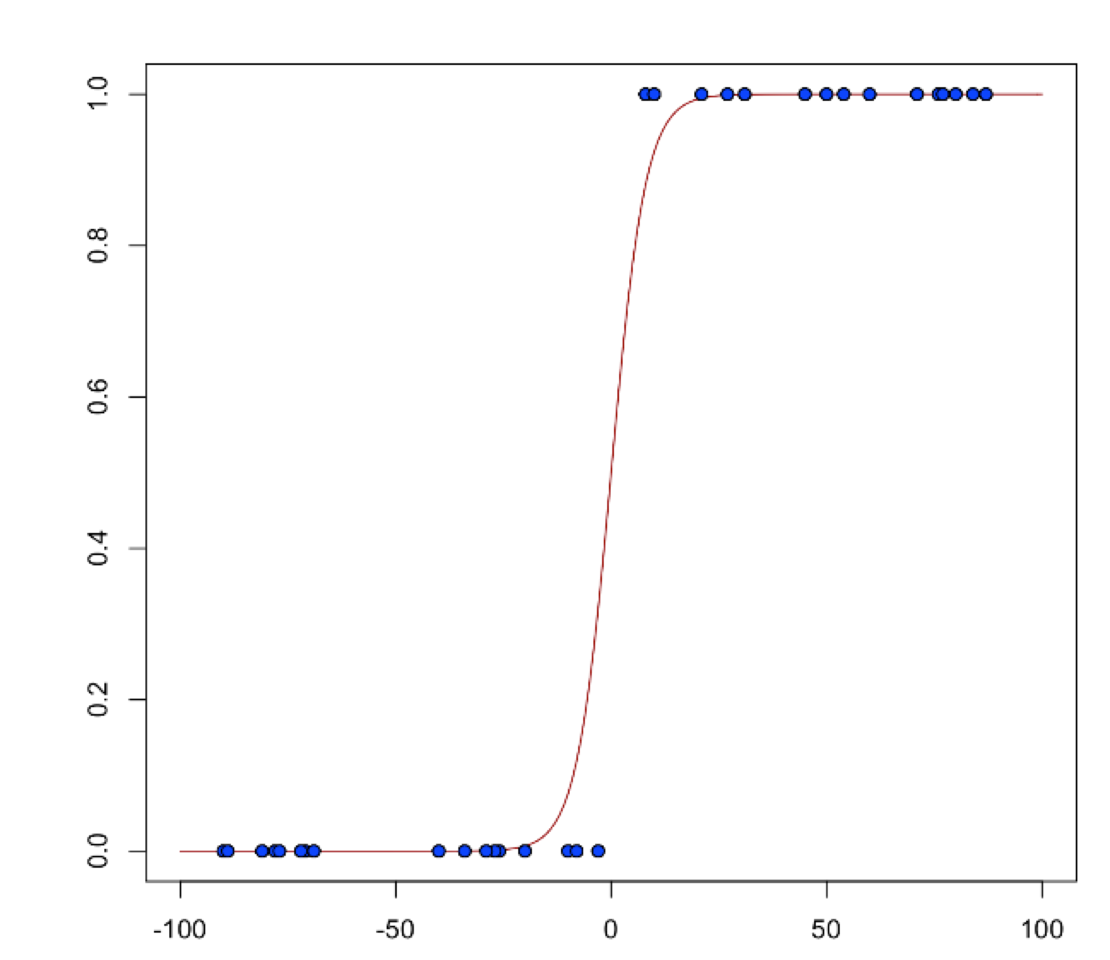
\includegraphics[scale=0.5]{images/scurve.png}
\end{figure}

and the fitted model has the form:
$$ \hat{y} = Pr(y = 1|x) = {e^{x^{\top}\beta + \beta_0} \over 1 + e^{x^{\top} \beta + \beta_0} }$$

This can alternatively be written as: 
$$  \log \left( \frac{\hat{y}}{ 1- \hat{y} } \right)  = \log \left(  \frac{Pr(y=1|x)}{Pr(y=0|x)}   \right) = x^{\top} \beta + \beta_0$$
%$$\log \left( \frac{\hat{y}}{ 1- \hat{y} } \right) = \log \left( \frac{Pr(y=1|x)}{Pr(y=0|x)} \right) = x^{\top} \beta + \beta_0.$$

The model is fitted by maximizing the following penalized likelihood: 
$$  \max_{\beta,\beta_0} \  \frac{1}{N} \sum_{i=1}^{N} \left( \ y_i (x_i^{\top}\beta  + \beta_0) - \log (1 + e^{x_i^{\top}\beta  + \beta_0} ) \right)  - \lambda \left( \alpha \|\beta \|_1 +  \frac{1}{2}(1- \alpha)  \| \beta \|_2^2 \right)$$

The corresponding deviance is equal to 
$$D = -2\sum_{i=1}^{n} \left(y_i \log(\hat{y}_i) + (1 - y_i)\log(1-\hat{y}_i)  \right).$$

Using the prostate dataset, this example builds a binomial model that classifies the incidence of penetration of the prostatic
capsule (CAPSULE). Confirm the entries in the CAPSULE column are binary using the \texttt{h2o.table()}
function. Change the regression by changing the family to binomial.

\waterExampleInR
\lstinputlisting[style=R]{GLM_Vignette_code_examples/glm_binomial_example.R}

\waterExampleInPython
\lstinputlisting[style=R]{GLM_Vignette_code_examples/glm_binomial_example.py}


\subsubsection{Logistic Ordinal Regression (Ordinal Family)}

A logistic ordinal regression model is a generalized linear model that predicts ordinal variables - variables that are discreet, as in classification, but that can be ordered, as in regression.

Let $X_i\in\rm \Bbb I \!\Bbb R^{p}$, $y$ can belong to any of the $K$ classes. In logistic ordinal regression, we model the cumulative distribution function (CDF) of $y$ belonging to class $j$, given $X_i$ as the logistic function:

$$P(y \leq j|X_i) = \phi(\beta^{T}X_i + \theta_j) = \dfrac {1} {1+ \text{exp} (-\beta^{T}X_i - \theta_j)}$$

Compared to multiclass logistic regression, all classes share the same $\beta$ vector. This adds the constraint that the hyperplanes that separate the different classes are parallel for all classes. To decide which class will $X_i$ be predicted, we use the thresholds vector $\theta$. If there are $K$ different classes, then $\theta$ is a non-decreasing vector (that is, $\theta_0 \leq \theta_1 \leq \ldots \theta_{K-2})$ of size $K-1$. We then assign $X_i$ to the class $j$ if $\beta^{T}X_i + \theta_j > 0$ for the lowest class label $j$.

We choose a logistic function to model the probability $P(y \leq j|X_i)$ but other choices are possible. 

To determine the values of $\beta$ and $\theta$, we maximize the log-likelihood minus the same Regularization Penalty, as with the other families. 

$$L(\beta,\theta) = \sum_{i=1}^{n} \text{log} \big( \phi (\beta^{T}X_i + \theta_{y_i}) - \phi(\beta^{T}X_i + \theta_{{y_i}-1}) \big)$$

Conventional ordinal regression uses a likelihood function to adjust the model parameters. However, during prediction, GLM looks at the log CDF odds. 

$$log \frac {P(y_i \leq j|X_i)} {1 - P(y_i \leq j|X_i)} = \beta^{T}X_i + \theta_{y_j}$$

As a result, there is a small disconnect between the two. To remedy this, we have implemented a new algorithm to set and adjust the model parameters. 

Recall that during prediction, a dataset row represented by $X_i$ will be set to class $j$ if 

$$log \frac {P(y_i \leq j|X_i)} {1 - P(y_i \leq j|X_i)} = \beta^{T}X_i + \theta_{j} > 0 $$

and

$$\beta^{T}X_i + \theta_{j'} \leq 0 \; \text{for} \; j' < j$$

Hence, for each training data sample $(X_{i}, y_i)$, we adjust the model parameters $\beta, \theta_0, \theta_1, \ldots, \theta_{K-2}$ by considering the thresholds $`\beta^{T}X_i + \theta_j$ directly. The following loss function is used to adjust the model parameters:

\begin{figure}[h]
\centering
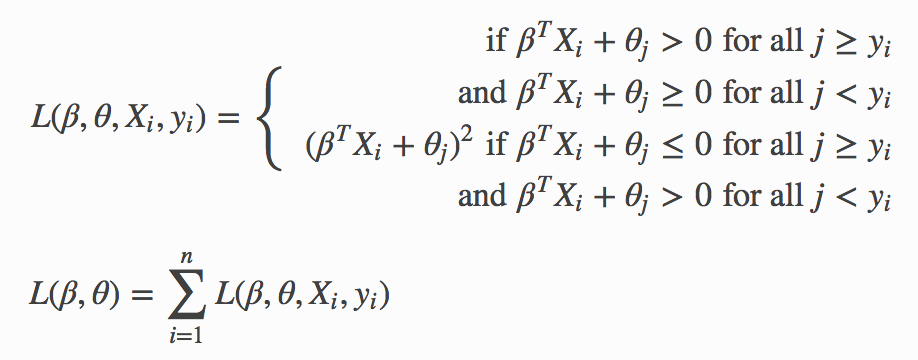
\includegraphics[scale=0.5]{images/ordinal_equation.png}
\end{figure}

Again, you can add the Regularization Penalty to the loss function. The model parameters are adjusted by minimizing the loss function using gradient descent. When the Ordinal family is specified, the \texttt{solver} parameter will automatically be set to \texttt{GRADIENT\_DESCENT\_LH} and use the log-likelihood function. To adjust the model parameters using the loss function, you can set the solver parameter to \texttt{GRADIENT\_DESCENT\_SQERR}. 

Because only first-order methods are used in adjusting the model parameters, use Grid Search to choose the best combination of the \texttt{obj\_reg}, \texttt{alpha}, and \texttt{lambda} parameters.

In general, the loss function methods tend to generate better accuracies than the likelihood method. In addition, the loss function method is faster as it does not deal with logistic functions - just linear functions when adjusting the model parameters.

\waterExampleInR
\lstinputlisting[style=python]{GLM_Vignette_code_examples/glm_ordinal_example.R}

\waterExampleInPython
\lstinputlisting[style=python]{GLM_Vignette_code_examples/glm_ordinal_example.py}

\subsubsection{Multi-class classification (Multinomial Family)}
Multinomial family generalization of the binomial model is used for multi-class response variables. Similar to the
binomial family, we model the conditional probability of observing class c given x. We have a vector of coefficients
for each of the output classes ($\beta$ is a matrix). The probabilities are defined as

$$ \hat{y}_c = Pr(y = c|x) = {e^{x^{\top}\beta_c + \beta_{c0}} \over \sum_{k=1}^K (e^{x^{\top}\beta_k + \beta_{k0}}) }$$ 

The penalized negative log-likelihood is defined as:

$$
- \lbrack {1\over{N}} \sum_{i=1}^N\sum_{k=1}^K(y_{i,k}(x_i^{\top}\beta_k + \beta_{k0})) - log(\sum_{k=1}^Ke^{x_i^{\top}\beta_k + \beta_{k0}}) \rbrack + \lambda \lbrack {(1-\alpha) \over 2} \| \beta \|_F^2 + \alpha\sum_{j=1}^P \|\beta_j\|_1 \rbrack 
$$
, where $\beta_c$ is vector of coefficients for class c and $y_{i,k}$ is kth element of the binary vector produced by
expanding the response variable using one-hot encoding (i.e. $y_{i,k} == 1$ iff the response at the ith observation
is k. It is 0 otherwise.

Here is a simple example using the iris dataset:


\waterExampleInR
\lstinputlisting[style=R]{GLM_Vignette_code_examples/glm_multinomial.R}

\waterExampleInPython
\lstinputlisting[style=python]{GLM_Vignette_code_examples/glm_multinomial.py}


\subsubsection{Poisson Models}
Poisson regression is typically used for datasets where the response represents counts and the errors are assumed to have a Poisson distribution. In general, it can be applied to any data where the response is non-negative. It models the dependency between the response and covariates as: 
%When building a Poisson model, we usually model dependency of the mean on the log scale, i.e. canonical link is log
%and prediction is:
\nowidow[3]

$$\hat{y} = e^{x^T\beta + \beta_0}$$

The model is fitted by maximizing the corresponding penalized likelihood:

$$  \max_{\beta,\beta_0}  \ \frac{1}{N} \sum_{i=1}^{N}  \left(   y_i (x_i^{\top}\beta  + \beta_0) - e^{x_i^{\top}\beta  + \beta_0} \right) 
- \lambda \left(\alpha \|\beta \|_1 + \frac{1}{2}(1-\alpha) \| \beta \|_2^2 \right)$$

The corresponding deviance is equal to: 

$$D = -2\sum_{i=1}^{N} \left( y_i \log(y_i/\hat{y}_i) - ( y_i - \hat{y}_i  ) \right)$$

Note in the equation above that H2O-3 uses the negative log of the likelihood. This is different than the way deviance is specified in \url{https://onlinecourses.science.psu.edu/stat501/node/377/}. In order to use this deviance definition, simply multiply the H2O-3 deviance by -1.

The following example loads the Insurance data from the MASS library, imports it into H2O, and runs a Poisson model that predicts the number of claims (Claims) based on the district of the policy holder (District), their age (Age), and the type of car they
own (Group).

\waterExampleInR
\lstinputlisting[style=R]{GLM_Vignette_code_examples/glm_poisson_example.R}

\waterExampleInPython
\lstinputlisting[style=python]{GLM_Vignette_code_examples/glm_poisson_example.py}

\subsubsection{Gamma Models}
The gamma distribution is useful for modeling a positive continuous response variable, where the conditional
variance of the response grows with its mean but the coefficient of variation of the response $\sigma^2(y_i)/\mu_i$ is
constant. It is usually used with the log link $g(\mu_i)= \log(\mu_i)$, or the inverse link $g(\mu_i) = \frac{1}{\mu_i} $ which is equivalent to the canonical link.

The model is fitted by solving the following likelihood maximization:

$$  \max_{\beta,\beta_0} \  - \frac{1}{N}  \sum_{i=1}^N  \ \frac{y_i}{x_i^{\top}\beta+\beta_0 } + \log(x_i^{\top}\beta + \beta_0) -\lambda \left(  \alpha \| \beta \|_1 + \frac{1}{2}(1-\alpha)\| \beta \|_2^2  \right) $$
%\[  \min\limits_{\beta,\beta_0} { {1 \over N}\sum\limits_{i=1}\limits^{N}{y_i \over (x_i^{T}\beta  + \beta_0)} - log({x_i^{T}\beta  + \beta_0})  + \lambda (\alpha \|\beta \|_1 + {1-\alpha \over 2}) \| \beta \|_2^2} \]

The corresponding deviance is equal to:

$$D = 2\sum_{i=1}^{N} - \log\left({\frac{ y_i }{\hat{y}_i}}\right) + \frac{(y_i - \hat{y}_i)}{\hat{y}_i} $$

To change the link function from the default inverse function to the log link function, modify the \texttt{link}
argument. 

\waterExampleInR

\lstinputlisting[style=R]{GLM_Vignette_code_examples/glm_gamma_example.R}

\waterExampleInPython
\lstinputlisting[style=python]{GLM_Vignette_code_examples/glm_gamma_example.py}

\subsubsection{Tweedie Models}

Tweedie distributions are a family of distributions which include gamma, normal, Poisson and their combination. It is especially useful for modeling positive continuous variables with exact zeros. The variance of the Tweedie distribution is proportional to the $p$-th power of the mean $var(y_i)=\phi \mu_i^p$. 

The Tweedie distribution is parametrized by variance power $p$. It is defined for all $p$ values except in the $(0,1)$ interval, and has the following distributions as special cases.

\begin{itemize}
\item  $p=0$: Normal
\item  $p=1$: Poisson
\item $p\in(1, 2)$: Compound Poisson, non-negative with mass at zero
\item $p=2$: Gamma
\item $p=3$: Inverse-Gaussian
\item $p>2$:  Stable, with support on the positive reals % (was 2?)
\end{itemize}

\waterExampleInR
\lstinputlisting[style=R]{GLM_Vignette_code_examples/glm_tweedie_example.R}

\newpage
\waterExampleInPython
\lstinputlisting[style=python]{GLM_Vignette_code_examples/glm_tweedie_example.py}

The normal and Poisson examples have already been covered in the previous sections. For $p>1$, the model likelihood to maximize has the form: 
$$  \max_{\beta,\beta_0} \ \sum_{i=1}^N \log(a(y_i,\phi)) + \left( \frac{1}{\phi}\left( \frac{y_i\mu_i^{1-p}}{1-p} - \kappa(\mu_i,p) \right)  \right) -\lambda  \left(  \alpha \| \beta \|_1 + \frac{1}{2}(1-\alpha)\| \beta \|_2^2  \right), $$
where $\kappa(\mu,p) = \mu^{2-p}/(2-p)$ for $p \neq 2$ and $\kappa(\mu,p) = \log(\mu)$ for $p=2$ and where the function $a(y_i,\phi)$ is evaluated using series expansion, since it does not have an analytical solution. The link function in the GLM representation of the Tweedie distribution defaults to $g(\mu) = \mu^{q} = \eta = X\beta$ with $q=1-p$. The link power $q$ can be set to other values, including $q=0$ which is interpreted as $\log(\mu)=\eta$. 
%
%have the form of the distribution \\
%link function can be taken as $\mu^{1-p}$ when p is not equal to 1\\
%giving: link $\mu=g^{-1}(\eta)$ or $\eta=X\beta = g(\mu)$ \\
%satisfies being the identity when p=0 cause $\eta = \mu^1$\\
%for p=2 satisfies the inverse link $\eta = \mu^-1$\\
%for $p=3$ satisfies the link which is the $inverse^2$ for the inverse gaussian.\\
%so when write the distribution for the tweedie we can replace $\mu$ by Ginverse of eta and we will have Xbeta in the expression. 
%Apart from the special cases, the density of the distribution does not have an analytic expression. The model likelihood to maximize is

The corresponding deviance when $p \neq 1$ and $p\neq 2$ is equal to:
$$D = 2\sum_{i}^N \frac{y_{i}(y_{i}^{1-p} - \hat{y}_{i}^{1-p})}{(1-p)} - \frac{(y_{i}^{2-p} - \hat{y}_{i}^{2-p})}{(2-p)} $$\\

%\waterExampleInR
%This example loads the Insurance data from the HDtweedie library, imports it into H2O and runs a tweedie model that predicts the aggregate claim loss (in thousand dollars) based on 56 predictors including the car type, job class etc.
%\lstinputlisting[style=R]{GLM_Vignette_code_examples/glm_tweedie_example.R}

%\waterExampleInPython
%\lstinputlisting[style=python]{GLM_Vignette_code_examples/glm_tweedie_example.py}

\subsubsection{Negative Binomial Models}

Negative binomial regression is a generalization of Poisson regression that loosens the restrictive assumption that the variance is equal to the mean. Instead, the variance of negative binomial is a function of its mean and parameter $\theta$, the dispersion parameter. 

Let $Y$ denote a random variable with negative binomial distribution, and let $\mu$ be the mean. The variance of $Y (\sigma^2)$ will be $\sigma^2 = \mu + \theta\mu^2$. The possible values of $Y$ are non-negative integers like 0, 1, 2, ...

The negative binomial regression for an observation $i$ is:

$$Pr(Y = y_i|\mu_i, \theta) = \frac{\Gamma(y_i+\theta^{-1})}{\Gamma(\theta^{-1})\Gamma(y_i+1)} {\bigg(\frac {1} {1 + {\theta {\mu_i}}}\bigg) ^\theta}^{-1} { \bigg(\frac {{\theta {\mu_i}}} {1 + {\theta {\mu_i}}} \bigg) ^{y_i}}$$

where $\Gamma(x)$ is the gamma function, and $\mu_i$ can be modeled as:

$$ \mu_i=\left\{
                \begin{array}{ll}
                  exp (\beta^T X_i + \beta_0) \text{  for log link}\\
                  \beta^T X_i + \beta_0 \text{  for identity link}\\
                \end{array}
              \right. $$

The  negative log likelihood $L(y_i,\mu_i)$ function is:

\begin{multline*}
$$^\text{max}_{\beta,\beta_0} \bigg[ \frac{-1}{N} \sum_{i=1}^{N}  \bigg \{ \bigg( \sum_{j=0}^{y_i-1} \text{log}(j + \theta^{-1} ) \bigg) - \text{log} (\Gamma (y_i + 1)) - (y_i + \theta^{-1}) \text{log} (1 + \alpha\mu_i) \\
+ y_i \text{log}(\mu_i) + y_i \text{log} (\theta) \bigg \} \bigg]$$
\end{multline*}

The final penalized negative log likelihood is used to find the coefficients $\beta, \beta_0$ given a fixed $\theta$ value:

$$ L(y_i, \mu_i) + \lambda \big(\alpha || \beta || _1 + \frac{1}{2} (1 - \alpha) || \beta || _2 \big)$$

The corresponding deviance is:

$$D = 2 \sum_{i=1}^{N} \bigg \{ y_i \text{log} \big(\frac{y_i}{\mu_i} \big) - (y_i + \theta^{-1}) \text{log} \frac{(1+\theta y_i)}{(1+\theta \mu_i)} \bigg \}$$

\textbf{Note}: Future versions of this model will optimize the coefficients as well as the dispersion parameter. Please stay tuned.

\newpage
\waterExampleInR
\lstinputlisting[style=R]{GLM_Vignette_code_examples/glm_negativebinomial_example.R}

\waterExampleInPython
\lstinputlisting[style=python]{GLM_Vignette_code_examples/glm_negativebinomial_example.py}

%----------------------------------------------------------------------
%----------------------------------------------------------------------

\section{Building GLM Models in H2O}

H2O's GLM implementation presents a high-performance distributed algorithm that scales linearly with the number
of rows and works extremely well for datasets with a limited number of active predictors.

\subsection{Classification and Regression}

GLM can produce two categories of models: classification (binary classification only) and regression. Logistic regression is the GLM to perform binary classification.

The data type of the response column determines the model category.  If the response is a categorical variable
(also called a factor or an enum), then a classification model is created.  If the response column data type is
numeric (either integer or real), then a regression model is created. 

The following examples show how to coerce the data type of a column to a factor.

\waterExampleInR
\lstinputlisting[style=R]{GLM_Vignette_code_examples/coerce_column_to_factor.R}

\waterExampleInPython
\lstinputlisting[style=python]{GLM_Vignette_code_examples/coerce_column_to_factor.py}

\subsection{Training and Validation Frames}

Frame refers to an H2OFrame, the fundamental method of data storage in H2O's distributed memory.

\texttt{training\_frame} refers to a frame containing a training dataset.  All predictors and the response (as
well as offset and weights, if specified) must be included in this frame.

\texttt{validation\_frame} refers to an optional frame containing a validation dataset.  If specified, this 
frame must have exactly the same columns as the training dataset.  Metrics are calculated on the validation dataset for convenience.

%If a validation dataset is not specified during training, there are functions that can calculate the same metrics after the model training is complete. %%would be helpful to provide examples or where users can find these functions. 

\subsection{Predictor and Response Variables}

Every model must specify its predictors and response.  Predictors and responses are specified by the $x$
and $y$ parameters.

$x$ contains the list of column names or column indices referring to vectors from the training frame; periods are not supported characters.

$y$ is a column name or index referring to a vector from the training frame.

\subsubsection{Categorical Variables}

If the response column is categorical, then a classification model is created.  GLM only supports binary
classification, so the response column may only have two levels. Categorical predictor columns may have more than two levels.

We recommend letting GLM handle categorical columns, as it can take advantage of the categorical
column for better performance and memory utilization.

We strongly recommend avoiding one-hot encoding categorical columns with many levels into many binary columns, as this is very inefficient.  This is especially true for Python users who are used to expanding their categorical variables manually for other frameworks.

\subsection{Family and Link}

Family and Link are optional parameters. The default family is \texttt{Gaussian} and the default link is a
canonical link for the selected family. These are passed as strings, e.g. \texttt{family = "gamma", link = "log"}.
While it is possible to select  a non-canonical link, this may lead to an unstable computation. 

\subsection{Regularization Parameters}

To get the best possible model, we need to find the optimal values of the regularization parameters $\alpha$ and
$\lambda$.  To find the optimal values, H2O provides grid search over $\alpha$ and a special form of grid search
called ``lambda search" over $\lambda$. For a detailed explanation, refer to {\textbf{\nameref{regularization}}}.

The recommended way to find optimal regularization settings on H2O is to do
a grid search over a few $\alpha$ values with an automatic lambda search for each $\alpha$. Both are described
below in greater detail.

\subsubsection{Alpha and Lambda}

The \texttt{alpha} parameter controls the distribution between  the $\ell_1$ (Lasso) and  $\ell_2$ (Ridge regression) penalties.  A value of 1.0 for \texttt{alpha} 
 represents Lasso, and an \texttt{alpha} value of 0.0 produces ridge regression.

The \texttt{lambda} parameter controls the amount of regularization applied.  If \texttt{lambda} is 0.0, no 
regularization is applied and the \texttt{alpha} parameter is ignored.  The default value for \texttt{lambda} is
calculated by H2O using a heuristic based on the training data.  If you let H2O calculate the value for \texttt{lambda}, you can see the chosen value in the model output.

\subsubsection{Lambda Search}
Lambda search enables efficient and automatic search for the optimal value of the \texttt{lambda} parameter. When lambda search is enabled, GLM will first fit a model with maximum regularization and then keep decreasing it until overfitting occurs. The resulting model is based on the best \texttt{lambda} value. 

When looking for sparse solution (\texttt{alpha} $>$ 0), lambda search can also be used to efficiently handle very wide datasets because it can filter out inactive predictors (known as noise) and only build models for a small subset of predictors. A common use of lambda search is to run it on a dataset with many predictors but limit the number of active predictors to a relatively small value.  

Lambda search can be enabled by setting \texttt{lambda\_search} and can be configured using the following arguments:

\begin{itemize}
\item \texttt{alpha}: Regularization distribution between  $\ell_1$ and  $\ell_2$.
\item \texttt{validation\_frame} and\/or \texttt{n\_folds}: Used to select the best lambda based on the cross-validation performance  or the validation or training data. If available, cross-validation performance takes precedence. If no validation data is available, the best lambda is selected based on training data performance and is therefore guaranteed to always be the minimal lambda computed, since GLM can not overfit on a training dataset.
 
\textbf{Note:} If running lambda search with a validation dataset and cross-validation disabled, the chosen lambda value corresponds to the lambda with the lowest validation error. The validation dataset is used to select the model and the model performance should be evaluated on another independent test dataset. 

\item \texttt{lambda\_min\_ratio} and \texttt{nlambdas}: The sequence of $\lambda$s is automatically generated as an exponentially decreasing sequence. It ranges from $\lambda_{max}$,
the smallest $\lambda$ so that the solution is a model with all 0s, to $\lambda_{min} =
$ \textit{lambda\_min\_ratio} * $ \lambda_{max}$.

H2O computes $\lambda$-models sequentially and in decreasing order, warm-starting the model for $\lambda_k$ with the solution for $\lambda_{k-1}$. By warm-starting (using the previous solution as the initial prediction) the models, we get better performance: typically models for subsequent $\lambda$s are close to each other, so only a few iterations per $\lambda$ are needed (typically two or three). This also achieves greater numerical stability, since models with a higher penalty are easier to compute. This method starts with an easy problem and then continues to make small adjustments. 

\textbf{Note:} \texttt{nlambda} and \texttt{lambda\_min\_ratio} also specify the relative distance of any two
 lambdas in the sequence. This is important when applying recursive strong rules, which are only effective if the neighboring lambdas are ``close" to each other. The default values are \texttt{nlambda} = 100 and $\lambda_{min}
= \lambda_{max} 1e^{-4}$, which gives us the ratio of 0.912.  For best results when using strong rules, keep the
ratio close to the default.

\item \texttt{max\_active\_predictors}: This limits the number of active predictors (the actual number of non-zero predictors in the model is going to be slightly lower). It is useful when obtaining a sparse solution to avoid costly computation of models with too many predictors.

\end{itemize}

\newpage
\subsection{Solver Selection}

This section provides general guidelines for best performance from the H2O GLM implementation options. The optimal solver depends on the data properties and prior information regarding the variables (if available). 

The data are considered sparse if the ratio of zeros to non-zeros in the input matrix is greater than $\sim 10$. The solution is sparse when only a subset of the original set of variables is intended to be kept in the model. In a dense solution, all predictors have non-zero coefficients in the final model.  

\subsubsection{Solver Details}
H2O's GLM offers the following solvers: 

\begin{itemize}
\item the Iteratively Reweighted Least Squares Method (IRLSM)
\item the Limited-memory Broyden-Fletcher-Goldfarb-Shanno algorithm (L-BFGS)
\item Coordinate Decent
\item Coordinate Decent Naive
\item Gradient Descent Likelihood (available for Ordinal family only; default for Ordinal family)
\item Gradient Descent Squared Error (available for Ordinal family only)
\end{itemize}

IRLSM uses a Gram Matrix approach, which is very efficient for tall and narrow datasets and when running lambda search with a sparse solution.  For wider and dense datasets (thousands of predictors and up), the L-BFGS solver scales better. If there are fewer than $\sim 500$ predictors in the data, use the default, which is IRLSM. 

For larger numbers of predictors, it is recommended to run IRLSM with lambda search and compare it to L-BFGS with just the $\ell_2$ penalty. For advanced users, we recommend the following general guidelines:
%H2O's GLM offers two different approaches for datasets with more than a thousand predictors.%depending on the expected number of coefficients to be included in the model: % to handling wide datasets: the IRLSM and the L-BFGS solvers.
\begin{itemize}
\item For a dense solution and a dense dataset, use IRLSM if there are fewer than $\sim 500$ predictors in the data; otherwise, use L-BFGS. Set \texttt{alpha} to 0 to include $\ell_2$ regularization in the elastic net penalty term to avoid inducing sparsity in the model.
   %   \texttt{alpha} equal to 0. This way only the $\ell_2$ regularization is included in the elastic net penalty term, and no sparsity is induced in the model. 
\item For a dense solution with a sparse dataset, use IRLSM if there are fewer than $\sim 2000$ predictors in the data; otherwise, use L-BFGS. Set \texttt{alpha} to 0.
%$< \  \sim5000$ predictors (i.e. one which only keeps some predictors in the final model), use the IRLSM solver with 
  %    \texttt{alpha} greater than 0. This adds an $\ell_1$ penalty to the elastic net regularization which induces sparsity in the estimated coefficients. Make sure \texttt{lambda\_search} is enabled to get models for the full regularization path. 
\item For a sparse solution with a dense dataset, use IRLSM with lambda-search if fewer than $\sim 500$ active predictors in the solution are expected; otherwise, use L-BFGS. Set \texttt{alpha} to be greater than zero to add an $\ell_1$ penalty to the elastic net regularization, which induces sparsity in the estimated coefficients. 
\item For a sparse solution with a sparse dataset, use IRLSM with lambda-search if you expect less than $\sim 5000$ active predictors in the solution; otherwise, use L-BFGS. Set \texttt{alpha} to be greater than zero. 
\item If unsure whether the solution should be sparse or dense, try both and a grid of alpha values. The optimal model can be picked based on its performance on the validation data (or alternatively the performance in cross-validation when not enough data is available to have a separate validation dataset).      
\end{itemize}

 The above recommendations are general guidelines; if the performance of the method seems slow, experiment with the available options. 

%\subsection{Solver Selection} %wide data want lambda search with alpha > 0 
%The two solvers provided in H2O are the Iteratively Reweighted Least Squares Method (IRLSM) and the Limited-memory Broyden-Fletcher-Goldfarb-Shanno algorithm (L-BFGS).  
%comment on using IRLSM with coordinate descent or with ADMM as in the IRLSM called algo?
IRLSM can be run with two algorithms to solve its innermost loop: ADMM and cyclical coordinate descent. The latter is used in glmnet. 

The method is able to handle large datasets well and deals efficiently with sparse features. It should improve the performance when the data contains categorical variables with a large number of levels, as it is implemented to deal with such variables in a parallelized way. 

Coordinate descent can be implemented with naive or covariance updates as explained in the glmnet paper. The covariance updates version is faster when $N>p$ and $p \sim 500$. 

For Ordinal regression problems, H2O provides options for Gradient Descent. Gradient Descent is a first-order iterative optimization algorithm for finding the minimum of a function. In H2O's GLM, conventional ordinal regression uses a likelihood function to adjust the model parameters. The model parameters are adjusted by maximizing the log-likelihood function using gradient descent. When the Ordinal family is specified, the solver parameter will automatically be set to GRADIENT\_DESCENT\_LH. To adjust the model parameters using the loss function, you can set the \texttt{solver} parameter to GRADIENT\_DESCENT\_SQERR.

\subsubsection{Stopping Criteria}

When using the $\ell_1$ penalty with lambda search, specify a value for the \\ \texttt{max\_active\_predictors} parameter to stop the search before it completes.  

Models built at the beginning of the lambda search have higher lambda values, consider fewer predictors, and take less time to calculate the model. 

Models built at the end of the lambda search have
lower lambda values, incorporate more predictors, and take a longer time to calculate the model. Set the \texttt{nlambdas} parameter for a lambda search to specify the number of models attempted across the search.

\waterExampleInR
\lstinputlisting[style=R]{GLM_Vignette_code_examples/glm_stopping_criteria.R}

\waterExampleInPython
\lstinputlisting[style=python]{GLM_Vignette_code_examples/glm_stopping_criteria.py}

%For performance reasons, we recommend not using any  $\ell_1$ penalty when using the L-BFGS solver, since
%model building can be slower. It is often better to run lambda search with the IRLSM solver instead.

\subsection{Advanced Features}

H2O's GLM has several advanced features to help build better models.
\subsubsection{Standardizing Data}

The \texttt{standardize} parameter, which is enabled by default, standardizes numeric columns to have zero mean and
unit variance.  This parameter must be enabled (using \texttt{standardize=TRUE}) to produce standardized coefficient magnitudes in the model output.

We recommend enabling standardization when using regularization (i.e. \texttt{lambda} chosen by H2O or greater than 0). Only advanced users should disable this.

\subsubsection{Auto-remove collinear columns}
Collinear columns can cause problems during model fitting. The preferred way to deal with collinearity is to add some
regularization (either L1, L2 or Elastic Net). This is the default H2O behavior. However, if you want a non-regularized
solution, you can choose to automatically remove collinear columns by setting the \texttt{remove\_collinear\_columns}
option.

This option can only be used with the \texttt{IRLSM} solver and no regularization. If selected, H2O will automatically
remove columns if it detects collinearity. Which columns are removed depends on the order of the columns in the vector
of coefficients (Intercept first, then categorical variables ordered by cadrinality from largest to smallest, and then
numbers).

\waterExampleInR
\lstinputlisting[style=R]{GLM_Vignette_code_examples/glm_remove_collinear_columns.R}


\subsubsection{P-Values}
Z-score, standard error and p-values are classical statistical measures of model quality. p-values are essentially
hypothesis tests on the values of each coefficient. A high p-value means that a coefficient is unreliable
(insiginificant) while a low p-value suggest that the coefficient is statistically significant.

You can request p-values by setting the \\\texttt{compute\_p\_values} option. It can only be used with the
\texttt{IRLSM} solver and no regularization. It is recommended that you also set the
\texttt{remove\_collinear\_columns} option. Otherwise, H2O will return an error if it detects collinearity in the dataset and p-values are requested. 

\textbf{Note:} GLM auto-standardizes the data by default (recommended). This changes the p-value of the constant term
(intercept).

\waterExampleInR
\lstinputlisting[style=R]{GLM_Vignette_code_examples/glm_p_values.R}


\subsubsection{K-fold Cross-Validation}

All validation values can be computed using either the training dataset (the default option) or using K-fold
cross-validation (\texttt{kfolds $> 1$)}. When $K$-fold cross-validation is enabled, H2O randomly splits data into $K$
equally-sized sections, trains each of the $K$ models on $K-1$ sections, and computes validation on the section that was not
used for training.

You can also specify the rows assigned to each fold using the\\ \texttt{fold\_assignment}
or \texttt{fold\_column} parameters.

\waterExampleInR
\lstinputlisting[style=R]{GLM_Vignette_code_examples/glm_cross_validation.R}

\waterExampleInPython
\lstinputlisting[style=python]{GLM_Vignette_code_examples/glm_cross_validation.py}

\newpage
\subsubsection{Grid Search Over Alpha}

Alpha search is not always necessary; changing its value to 0.5 (or 0 or 1 if we only want Ridge or Lasso,
respectively) works in most cases. If $\alpha$ search is required, specifying only a few values is typically sufficient. Alpha
search is invoked by supplying a list of values for $\alpha$ instead of a single value. H2O then produces one model
per $\alpha$ value. 

The grid search computation can be done in parallel (depending on the cluster resources) and it
is generally more efficient than computing different models separately from R.

Use caution when including $\alpha=0$ or $\alpha=1$ in the grid search. $\alpha=0$ will produce a dense solution
and it can be very slow (or even impossible) to compute in large $N$ situations. $\alpha=1$ has no  $\ell_2$ penalty, so
it is therefore less numerically stable and can be very slow as well due to slower convergence. In general, we recommend using $alpha=1-\epsilon$ instead.

\waterExampleInR
\lstinputlisting[style=R]{GLM_Vignette_code_examples/glm_grid_search_over_alpha.R}

\newpage
\waterExampleInPython
\lstinputlisting[style=python]{GLM_Vignette_code_examples/glm_grid_search_over_alpha.py}

\subsubsection{Grid Search Over Lambda}

 While automatic lambda search is the preferred method,  a grid search over lambda values is also supported
 by passing in a vector of lambdas and disabling the lambda-search option. The behavior will be identical to lambda
 search, except H2O will use the specified list of lambdas instead (still capped at $\lambda_{max}$).

\waterExampleInR
\lstinputlisting[style=R]{GLM_Vignette_code_examples/glm_grid_search_over_lambda.R}

\waterExampleInPython
\lstinputlisting[style=python]{GLM_Vignette_code_examples/glm_grid_search_over_lambda.py}

%Grid search over lambda is a feature from H2O-2 that is not currently supported in H2O-3.  Instead, use the built-in lambda search capability in GLM.

\subsubsection{Offsets}

\texttt{offset\_column} is an optional column name or index referring to a column in the training frame. This column specifies a prior known component to be included in the linear predictor during training. Offsets are per-row "bias values" that are used during model training. 

For Gaussian distributions, they can be seen as simple corrections to the response (\texttt{y}) column. Instead of learning to predict the response (\texttt{y}-row), the model learns to predict the (row) offset of the response column. 

For other distributions, the offset corrections are applied in the linearized space before applying the inverse link function to get the actual response values.  

\subsubsection{Row Weights}
\texttt{weights\_column} is an optional column name or index referring to a column in the training frame. This column specifies on a per-row basis the weight of that row.  If no weight column is specified, a default value of 1 is used for each row. Weights are per-row observation weights. This is typically the number of times a row is repeated, but non-integer values are supported as well. During training, rows with higher weights matter more, due to the larger loss function pre-factor.

\subsubsection{Coefficient Constraints}
Coefficient constraints allow you to set special conditions over the model coefficients. Currently supported
constraints are upper and lower bounds and the proximal operator interface, as described in \citetalias{prox}.

The constraints are specified as a frame with following vecs (matched by name; all vecs can be sparse):

\begin{itemize}
\item \texttt{names}: (mandatory) coefficient names
\item \texttt{lower\_bounds}: (optional) coefficient lower bounds , must be less than or equal to \texttt{upper\_bounds}
\item \texttt{upper\_bounds}: (optional) coefficient upper bounds , must be greater than or equal to \texttt{lower\_bounds}
\item \texttt{beta\_given}: (optional) specifies the given solution in proximal operator interface
\item \texttt{rho}: (mandatory if \texttt{beta\_given} is specified, otherwise ignored): specifies per-column  $\ell_2$ penalties on the distance from the given solution
\item \texttt{mean}: specifies the mean override (for data standardization)
\item \texttt{std\_dev}: specifies the standard deviation override (for data standardization)
\end{itemize}
 
\subsubsection{Proximal Operators}

The proximal operator interface allows you to run the GLM with a proximal penalty on a distance from a specified
given solution. There are many potential uses: for example, it can be used as part of an ADMM consensus algorithm
to obtain a unified solution over separate H2O clouds or in Bayesian regression approximation.



%----------------------------------------------------------------------
%----------------------------------------------------------------------

\section{GLM Model Output}

The following sections represent the output produced by logistic regression (i.e. binomial classification).

\waterExampleInR
\lstinputlisting[style=R]{GLM_Vignette_code_examples/glm_model_output_10.R}

\newpage
\waterExampleInPython
\lstinputlisting[style=python]{GLM_Vignette_code_examples/glm_model_output_10.py}

\begin{lstlisting}[style=output]
Model Details:
==============

H2OBinomialModel: glm
Model ID:  GLM_model_R_1439511782434_25 
GLM Model:
    family  link                                regularization number_of_predictors_total number_of_active_predictors number_of_iterations training_frame
1 binomial logit Elastic Net (alpha = 0.5, lambda = 4.674E-4 )                          4                           5                    5      subset_39

Coefficients:
      names coefficients standardized_coefficients
1 Intercept    -6.467393                 -0.414440
2       AGE    -0.021983                 -0.143745
3      RACE    -0.295770                 -0.093423
4       PSA     0.028551                  0.604644
5   GLEASON     1.156808                  1.298815

H2OBinomialMetrics: glm
** Reported on training data. **

MSE:  0.1735008
R^2:  0.2842015
LogLoss:  0.5151585
AUC:  0.806806
Gini:  0.6136121
Null Deviance:  403.9953
Residual Deviance:  307.0345
AIC:  317.0345

Confusion Matrix for F1-optimal threshold:
         0   1    Error     Rate
0      125  50 0.285714  =50/175
1       24  99 0.195122  =24/123
Totals 149 149 0.248322  =74/298

Maximum Metrics:
                      metric threshold    value idx
1                     max f1  0.301518 0.727941 147
2                     max f2  0.203412 0.809328 235
3               max f0point5  0.549771 0.712831  91
4               max accuracy  0.301518 0.751678 147
5              max precision  0.997990 1.000000   0
6           max absolute_MCC  0.301518 0.511199 147
7 max min_per_class_accuracy  0.415346 0.739837 134

H2OBinomialMetrics: glm
** Reported on validation data. **

MSE:  0.1981162
R^2:  0.1460683
LogLoss:  0.5831277
AUC:  0.7339744
Gini:  0.4679487
Null Deviance:  108.4545
Residual Deviance:  95.63294
AIC:  105.6329

Confusion Matrix for F1-optimal threshold:
        0  1    Error    Rate
0      35 17 0.326923  =17/52
1       8 22 0.266667   =8/30
Totals 43 39 0.304878  =25/82

Maximum Metrics:
                      metric threshold    value idx
1                     max f1  0.469237 0.637681  38
2                     max f2  0.203366 0.788043  63
3               max f0point5  0.527267 0.616438  28
4               max accuracy  0.593421 0.719512  18
5              max precision  0.949357 1.000000   0
6           max absolute_MCC  0.469237 0.391977  38
7 max min_per_class_accuracy  0.482906 0.692308  36
\end{lstlisting}

\subsection{Coefficients and Normalized Coefficients}

Coefficients are the predictor weights (i.e. the actual model used for prediction).  Coefficients should be used to
make predictions for new data points:

\lstinputlisting[style=R]{GLM_Vignette_code_examples/glm_model_output_20.R}
\lstinputlisting[style=Python]{GLM_Vignette_code_examples/glm_model_output_20.py}
\begin{lstlisting}[style=output]
  Intercept         AGE        RACE         PSA     GLEASON 
-6.46739299 -0.02198278 -0.29576986  0.02855057  1.15680761 
\end{lstlisting}

If the \texttt{standardize} option is enabled, H2O returns another set of coefficients: the standardized
coefficients. These are the predictor weights of the standardized data and are included only for informational
purposes (e.g. to compare relative variable importance). 

In this case, the ``normal'' coefficients are obtained
from the standardized coefficients by \textbf{reversing} the data standardization process (de-scaled, with the
intercept adjusted by an added offset) so that they can be applied to data in its original form (i.e. no
standardization prior to scoring). \textbf{Note:} These are \textbf{not} the same as coefficients of a model built
on non-standardized data.

Standardized coefficients are useful for comparing the relative contribution of different predictors to the
model:

\lstinputlisting[style=R]{GLM_Vignette_code_examples/glm_model_output_30.R}
\lstinputlisting[style=Python]{GLM_Vignette_code_examples/glm_model_output_30.py}
\begin{lstlisting}[style=output]
Coefficients:
      names coefficients standardized_coefficients
1 Intercept    -6.467393                 -0.414440
2       AGE    -0.021983                 -0.143745
3      RACE    -0.295770                 -0.093423
4       PSA     0.028551                  0.604644
5   GLEASON     1.156808                  1.298815
\end{lstlisting}

This view provides a sorted list of standardized coefficients in descending order for easy comparison:

\lstinputlisting[style=R]{GLM_Vignette_code_examples/glm_model_output_40.R}
\lstinputlisting[style=Python]{GLM_Vignette_code_examples/glm_model_output_40.py}
\begin{lstlisting}[style=output]
Standardized Coefficient Magnitudes:
          names coefficients sign
GLEASON GLEASON     1.298815  POS
PSA         PSA     0.604644  POS
AGE         AGE     0.143745  NEG
RACE       RACE     0.093423  NEG
\end{lstlisting}

\subsection{Model Statistics}

Various model statistics are available:

\texttt{MSE} is the mean squared error: $MSE = {1 \over N} \sum_{i=1}^N (actual_i - prediction_i)^2$

\texttt{R\textasciicircum2} is the R squared: $R^2 = 1 - {MSE \over \sigma_y^2}$

\texttt{LogLoss} is the log loss. $LogLoss = {-1 \over N} \sum_i^N \sum_j^C y_{i}log(p_{i,j})$

\texttt{AUC} is available only for binomial models and is defined the area under ROC curve.

%\texttt{Gini}  TODO

\texttt{Null deviance} Deviance (defined by selected family) computed for the null model. 

\texttt{Residual deviance} Deviance of the built model

\texttt{AIC} is based on log-likelihood, which is summed up similarly to deviance

Retrieve these statistics using the following accessor functions:

\waterExampleInR
\lstinputlisting[style=R]{GLM_Vignette_code_examples/glm_accessors.R}

\waterExampleInPython
\lstinputlisting[style=python]{GLM_Vignette_code_examples/glm_accessors.py}

\subsection{Confusion Matrix}

Fetch the confusion matrix directly using the following accessor function:

\waterExampleInR
\lstinputlisting[style=R]{GLM_Vignette_code_examples/glm_confusion_matrix.R}


\waterExampleInPython
\lstinputlisting[style=python]{GLM_Vignette_code_examples/glm_confusion_matrix.py}

\subsection{Scoring History}

The following output example represents a sample scoring history: 

\lstinputlisting[style=R]{GLM_Vignette_code_examples/glm_scoring_history.R}
\waterExampleInPython
\lstinputlisting[style=python]{GLM_Vignette_code_examples/glm_scoring_history.py}
\begin{lstlisting}[style=output]
Scoring History:
            timestamp   duration iteration log_likelihood objective
1 2015-08-13 19:05:17  0.000 sec         0      201.99764   0.67784
2 2015-08-13 19:05:17  0.002 sec         1      158.46117   0.53216
3 2015-08-13 19:05:17  0.003 sec         2      153.74404   0.51658
4 2015-08-13 19:05:17  0.004 sec         3      153.51935   0.51590
5 2015-08-13 19:05:17  0.005 sec         4      153.51723   0.51590
6 2015-08-13 19:05:17  0.006 sec         5      153.51723   0.51590
\end{lstlisting}



%----------------------------------------------------------------------
%----------------------------------------------------------------------

\section{Making Predictions}

Once you have built a model, you can use it to make predictions using two different approaches:  the in-H2O batch scoring approach and the real-time nano-fast POJO approach.

\subsection{Batch In-H2O Predictions}

Batch in-H2O predictions are made using a normal H2O cluster on a new H2OFrame.  When you use \texttt{h2o.predict()}, the order of the rows in the results is the same as the order in which the data was loaded, even if some rows fail (for example, due to missing values or unseen factor levels). 
In addition to predictions, you can view metrics such as area under curve (AUC) if you include the response column in the new data.  The following example represents a logistic regression model (i.e. binomial classification).

\waterExampleInR

\lstinputlisting[style=R]{GLM_Vignette_code_examples/glm_binomial_predictions_with_response.R}


\waterExampleInPython
\lstinputlisting[style=python]{GLM_Vignette_code_examples/glm_binomial_predictions_with_response.py}

\newpage
Here is an example of making predictions on new data:

\waterExampleInR
\lstinputlisting[style=R]{GLM_Vignette_code_examples/glm_binomial_predictions_without_response.R}

\waterExampleInPython
\lstinputlisting[style=python]{GLM_Vignette_code_examples/glm_binomial_predictions_without_response.py}
\begin{lstlisting}[style=output]
  predict        p0        p1
1       1 0.1676892 0.8323108
2       0 0.4824181 0.5175819
3       1 0.2000061 0.7999939
4       0 0.9242169 0.0757831
5       0 0.5044669 0.4955331
6       0 0.7272743 0.2727257
\end{lstlisting}


The three columns in the prediction file are the predicted class, the probability that the prediction is class 0,
and the probability that the prediction is class 1. The predicted class is chosen based on the maximum-F1 threshold.

You can change the threshold manually, for example to 0.3, and recalculate the predict column like this:

\lstinputlisting[style=R]{GLM_Vignette_code_examples/glm_recalculate_predict.R}
\lstinputlisting[style=python]{GLM_Vignette_code_examples/glm_recalculate_predict.py}
\begin{lstlisting}[style=output]
  predict        p0        p1
1       1 0.1676892 0.8323108
2       1 0.4824181 0.5175819
3       1 0.2000061 0.7999939
4       0 0.9242169 0.0757831
5       1 0.5044669 0.4955331
6       0 0.7272743 0.2727257
\end{lstlisting}

\subsection{Low-latency Predictions using POJOs}

For nano-fast scoring, H2O GLM models can be directly rendered as a Plain Old Java Object (POJO).  POJOs are very
low-latency and can easily be embedded in any Java environment (a customer-facing web application, a Storm bolt,
or a Spark Streaming pipeline, for example).

The POJO does nothing but pure math, and has no dependencies on any other software packages (not even H2O),
so it is easy to implement.

Directions for using the POJO in detail are beyond the scope of this document, but the following example demonstrates how to generate and view a POJO.  To access the POJO from the Flow Web UI, click the \textsc{Download POJO} button at the bottom of the cell containing the generated model.

For more information on how to use an H2O POJO, refer to the \textbf{POJO Quick Start Guide} at {\url{https://github.com/h2oai/h2o-3/blob/master/h2o-docs/src/product/howto/POJO_QuickStart.md}}. 

\waterExampleInR
\lstinputlisting[style=R]{GLM_Vignette_code_examples/glm_download_pojo.R}
\newpage
\waterExampleInPython
\lstinputlisting[style=Python]{GLM_Vignette_code_examples/glm_download_pojo.py}

%----------------------------------------------------------------------
%----------------------------------------------------------------------

\section{Best Practices}

Here are a few rules of thumb to follow:

\begin{itemize}
\item Use symmetric nodes in your H2O cluster
\item Impute data before running GLM
\item The IRLSM solver works best on tall and skinny datasets
\item If you have a wide dataset, use an  $\ell_1$ penalty to eliminate columns from the model
\item If you have a wide dataset, use the L-BFGS solver
\item When using lambda search, specify a value for \texttt{max\_predictors} if the process takes too long. 90\% of the time is spent on the larger models with the small lambdas, so specifying \texttt{max\_predictors} can reduce this time
\item Retain a small  $\ell_2$ penalty (i.e. ridge regression) for numerical stability (i.e. don`t use \texttt{alpha} 1.0, use 0.95 instead)
\item When using the IRLSM solver, larger nodes can help the ADMM (Cholesky decomposition) run faster
\end{itemize}

\newpage
\subsection{Verifying Model Results}

To determine the accuracy of your model, use the following guidelines: 

\begin{itemize}
\item Look for conspicuously different cross-validation results between folds:

\waterExampleInR
\lstinputlisting[style=R]{GLM_Vignette_code_examples/glm_compare_cross_validation_folds.R}


\waterExampleInPython
\lstinputlisting[style=python]{GLM_Vignette_code_examples/glm_compare_cross_validation_folds.py}

\item Look for explained deviance ($1 - {NullDev - ResDev \over NullDev}$) 
      \begin{itemize}
      \item Too close to 0:  model doesn`t predict well (underfitting)
      \item Too close to 1:  model predicts too well due to noisy data (overfitting)
      \end{itemize}


\item For logistic regression (i.e. binomial classification) models, look for AUC
      \begin{itemize}
      \item Too close to 0.5:  model doesn`t predict well (underfitting)
      \item Too close to 1:  model predicts too well due to noisy data (overfitting)
      \end{itemize}
\item Look at the number of iterations  or scoring history to see if GLM stops early for a specific
      lambda; performing all the iterations usually means the solution is not good.  This is
      controlled by the \texttt{max\_iterations} parameter.
\item The fewer the NA values in your training data, the better; GLM will either skip or mean-impute rows with NA values. Always check degrees of freedom in the output model. Degrees of freedom is the number of observations used to train the model minus the size of the model. If this number is much smaller than expected, it is likely that too many rows have been excluded due to missing values. 

      \begin{itemize}
      \item If you have few columns with many NAs, you might accidentally be losing all your rows, so it`s better to exclude them.
      \item If you have many columns with small fraction of uniformly-distributed missing values, every row will likely have at least one missing value. In this case, impute the NAs (e.g. substituted with mean values) before modeling.
      \end{itemize}
\end{itemize}
%----------------------------------------------------------------------
%----------------------------------------------------------------------
\section{Implementation Details}

The following sections discuss some of the implementation choices in H2O's GLM.

\subsection{Categorical Variables}

When applying linear models to datasets with categorical variables, the usual approach is to expand the
categoricals into a set of binary vectors, with one vector per each categorical level (e.g. by calling
{\texttt{model.matrix}} in R). H2O performs similar expansions automatically and no prior changes to the dataset
are needed. Each categorical column is treated as a set of sparse binary vectors.

\subsubsection{Largest Categorical Speed Optimization}

Categoricals have special handling during GLM computation as well. When forming the gram matrix, we can take
advantage of the fact that columns belonging to the same categorical never co-occur and the gram matrix region
belonging to these columns will not have any non-zero elements outside of the diagonal. 

This keeps it in sparse representation, taking only $O(N)$ elements instead of $O(N*N)$. Furthermore, the complexity of Choelsky
decomposition of a matrix that starts with a diagonal region can be greatly reduced. H2O's GLM exploits these two
facts to handle the largest categorical ``for free". Therefore, when analyzing the performance of GLM in the
equation expressed above, we can subtract the size of the largest categoricals from the number of predictors.

$$N = \sum_{c \in C} (\|c.domain\|) - \arg\max_{c \in C} \|c.domain\| + \|Nums\| $$

\subsection{Performance Characteristics}

This section discusses the CPU and memory cost of the IRLSM and L-BFGS solvers for running GLM.

\subsubsection{IRLSM Solver}

The implementation is based on iterative re-weighted least squares with an ADMM inner solver (as described
in \citetalias{admm}) to deal with the  $\ell_1$ penalty. Every iteration of the algorithm consists of following steps:

\begin{enumerate} 
\item Generate weighted least squares problem based on previous solution, i.e. vector of weights $w$ and response $z$ 
\item Compute the weighted gram matrix $X^TWX$ and $X^Tz$ vector
\item Decompose the gram matrix (Cholesky decomposition) and apply ADMM solver to solve the  $\ell_1$ penalized least squares problem
\end{enumerate}

Steps 1 and 2 are performed distributively. Step 3 is computed in parallel on a single node. This method
characterizes the computational complexity and scalability of a dataset with $M$ observations and $N$ columns (predictors) on a cluster with $n$ nodes with $p$ CPUs each.

\bigskip

\begin{adjustbox}{width=\textwidth}%resizes table to text width
\centering % used for centering table 
    \begin{tabular}{ c || c | c }
        & & \\
        & CPU & Memory \\
        & & \\
        \hline
        \hline
        & & \\

        \begin{tabular}{@{}c@{}}Gram matrix ($ X^TX $) \\ (distributed)\end{tabular} &
        $ O(\dfrac{MN^2}{pn}) $ &
        \begin{tabular}{@{}c@{}} $O($training data$)$ + $O($gram matrix$)$ \\ $ O(MN) $ + $ O(N^2pn) $ \end{tabular}
        \\

        & & \\
        \hline
        & & \\

        \begin{tabular}{@{}c@{}}ADMM + Cholesky decomposition \\ (single node)\end{tabular} &
        $ O(\dfrac{N^3}{p}) $ &
        $ O(N^2) $
        \\

        & & \\

    \end{tabular}
\end{adjustbox}

    \begin{tabular}{ l l }

    $M$ & Number of rows in the training data \\
    $N$ & Number of predictors in the training data \\
    $p$ & Number of CPUs per node \\
    $n$ & Number of nodes in the cluster \\
    \end{tabular}


If $M>>N$, the algorithm scales linearly both in the number of nodes and the number of CPUs per node. However,
the algorithm is limited in the number of predictors it can handle, since the size of the Gram matrix grows
quadratically, due to a memory and network throughput issue with the number of predictors. 

Its decomposition
cost grows as the cube of the number of predictors increases, which is a computational cost issue. In many cases, H2O can work around these limitations due to its handling of categoricals and by employing strong rules to filter out inactive predictors.

\subsubsection{L-BFGS solver}
In each iteration, L-BFGS computes a gradient at the current vector of coefficients and then computes an updated vector of coefficients in an approximated Newton-method step. 

The cost of the coefficient update is $k*N$. $N$ is the number of predictors; $k$ is a constant. The cost of gradient computation is $M*N\over pn$ where $M$ is number of observations in the dataset and $pn$ is the number of CPU cores in the cluster. Since $k$ is a small constant, the runtime of L-BFGS is dominated by the gradient computation, which is fully parallelized, scaling L-BFGS almost linearly. 

\subsection{FAQ}

\begin{itemize}
\item \textbf{What if the training data contains NA values?}

 The rows with missing response are ignored during model training and validation.

\item \textbf{What if the testing data contains NA values?}

 If the missing value handling is set to skip and you are generating predictions, skipped rows will have NA (missing) prediction.

\item \textbf{What if, while making predictions on testing data, a predictor column is categorical and the predictor is a level not observed during training?}

 The value is zero for all predictors associated with that categorical variable.

\item \textbf{What if, while making predictions on testing data, the response column is categorical and the response is a level not observed during training?} 

H2O supports binomial models only; any extra levels in the test response will generate an error.
\end{itemize}

\section{Appendix: Parameters}
\begin{itemize}
\item \texttt{x}: A vector containing the names of the predictors to use while building the GLM model. No default.
\item \texttt{y}: A character string or index that represents the response variable in the model. No default.
\item \texttt{training\_frame}: An \texttt{H2OFrame} object containing the variables in the model. 
\item \texttt{model\_id}: (Optional) The unique ID assigned to the generated model. If not specified, an ID is generated automatically.
\item \texttt{validation\_frame}: An \texttt{H2OParsedData} object containing the validation dataset used to construct confusion matrix. If  blank, the training data is used by default.
\item \texttt{max\_iterations}: A non-negative integer specifying the maximum number of iterations. 
\item \texttt{objective\_epsilon}: Specify a threshold for convergence. If the objective value is less than this threshold, the model is converged.
\item \texttt{beta\_epsilon}: A non-negative number specifying the magnitude of the maximum difference between the coefficient estimates from successive iterations. Defines the convergence criterion. 
\item \texttt{gradient\_epsilon}: (For L-BFGS only) Specify a threshold for convergence. If the objective value (using the L-infinity norm) is less than this threshold, the model is converged.
\item \texttt{solver}: A character string specifying the solver used. \texttt{IRLSM} supports more features. \texttt{L\_BFGS} scales better for datasets with many columns. \texttt{COORDINATE\_DESCENT} is \texttt{IRLSM} with the covariance updates version of cyclical coordinate descent in the innermost loop. \\ \texttt{COORDINATE\_DESCENT\_NAIVE} is \texttt{IRLSM} with the naive updates version of cyclical coordinate descent in the innermost loop. \\ \texttt{GRADIENT\_DESCENT\_LH} and \\\texttt{GRADIENT\_DESCENT\_SQERR} can only be used with the Ordinal family.
\item \texttt{standardize}: A logical value that indicates whether the numeric predictors should be standardized to have a mean of 0 and a variance of 1 prior to model training. 
\item \texttt{family}: A description of the error distribution and corresponding link function to be used in the model. The following options are supported: \texttt{gaussian} (default), \texttt{binomial}, \texttt{gamma}, \texttt{ordinal}, \texttt{multinomial}, \texttt{poisson}, \texttt{tweedie,} \texttt{quasibinomial}, or \texttt{negativebinomial}. When a model is specified as Tweedie, users must also specify the appropriate Tweedie power. %%need to specify `tweedie_variance_power` and `tweedie_link_power`??
\item \texttt{link}: The link function relates the linear predictor to the distribution function. The default is the canonical link for the specified family. The full list of supported links for each family: 
	\begin{itemize}
\item	{\textbf {logit}}: binomial, quasibinomial
\item {\textbf{identity}}: gaussian, poisson, gamma, negativebinomial
\item {\textbf{log}}: gaussian, negativebinomial
\item {\textbf{inverse}}: gaussian, gamma
\item {\textbf{tweedie}}: tweedie
\item {\textbf{multinomial}} (family\_default): multinomial 
\item {\textbf{ordinal}}: ologit, oprobit, and ologlog
	\end{itemize}
\item \texttt{tweedie\_variance\_power}: A numeric specifying the power for the variance function when \texttt{family = "tweedie"}.  Default is 0.
\item \texttt{tweedie\_link\_power}: A numeric specifying the power for the link function when \texttt{family = "tweedie"}.  Default is 1.
\item \texttt{theta}: Theta value (equal to 1/r) for use with the negative binomial family. This value must be \textgreater 0 and defaults to 1e-10.
\item \texttt{alpha}: The elastic-net mixing parameter, which must be in $[0,1]$. The penalty is defined to be $P(\alpha,\beta) = (1-\alpha)/2||\beta||_2^2 + \alpha||\beta||_1 = \sum_j [(1-\alpha)/2 \beta_j^2 + \alpha|\beta_j|] $ so \texttt{alpha=1} is the Lasso penalty, while \texttt{alpha=0} is the ridge penalty. Default is 0.5.
\item \texttt{prior}: (Optional) A numeric specifying the prior probability of class 1 in the response when \texttt{family = "binomial"}. The default value is the observation frequency of class 1. Must be from (0,1) exclusive range or NULL (no prior).
\item \texttt{lambda}: A non-negative value representing the shrinkage parameter, which multiplies $P(\alpha,\beta)$ in the objective. The larger lambda is, the more the coefficients are shrunk toward zero (and each other). When the value is 0, regularization is disabled and ordinary generalized linear models are fit. The default is 1e-05.
\item \texttt{lambda\_search}: A logical value indicating whether to conduct a search over the space of lambda values, starting from the max lambda, given lambda will be interpreted as the min. lambda. Default is false.
\item \texttt{nlambdas}: The number of lambda values when \texttt{lambda\_search = TRUE}. Default is -1.
\item \texttt{lambda\_min\_ratio}: Smallest value for lambda as a fraction of \\ lambda.max, the entry value, which is the smallest value for which all coefficients in the model are zero. If the number of observations is greater than the number of variables then \texttt{lambda\_min\_ratio = 0.0001}; if the number of observations is less than the number of variables then \texttt{lambda\_min\_ratio = 0.01}. Default is -1.0.
\item \texttt{nfolds}: Number of folds for cross-validation. If \texttt{nfolds >=2}, then \texttt{validation\_frame} must remain blank. Default is 0. %%validation_frame = correct? just says "validation" in R doc...
\item \texttt{fold\_column}: (Optional) Column with cross-validation fold index assignment per observation. 
\item \texttt{fold\_assignment}: Cross-validation fold assignment scheme, if \\ \texttt{fold\_column} is not specified. The following options are supported: \texttt{AUTO, Random,} or \texttt{Modulo}. 
\item \texttt{keep\_cross\_validation\_predictions}: Specify whether to keep the predictions of the cross-validation models. 
\item \texttt{beta\_constraints}: A data frame or \texttt{H2OParsedData} object with the columns \texttt{["names", "lower\_bounds", "upper\_bounds", \\ "beta\_given"]}, where each row corresponds to a predictor in the GLM. \texttt{"names"} contains the predictor names, \texttt{"lower\_bounds"/ \\ "upper\_bounds"} are the lower and upper bounds (respectively) of the beta, and  \texttt{"beta\_given"} is a user-specified starting value. 
\item \texttt{offset\_column}: Specify the offset column. Note: Offsets are per-row “bias values” that are used during model training. For Gaussian distributions, they can be seen as simple corrections to the response (y) column. Instead of learning to predict the response (y-row), the model learns to predict the (row) offset of the response column. For other distributions, the offset corrections are applied in the linearized space before applying the inverse link function to get the actual response values. 
\item \texttt{weights\_column}: Specify the weights column. These are per-row observation weights. This is typically the number of times a row is repeated. Non-integer values are also supported. During training, rows with higher weights matter more, due to the larger loss function pre-factor.
\item \texttt{intercept}: Logical; includes a constant term (intercept) in the model. Must be included if there are factor columns in your model. %% <--- still true? copied from `has_intercept`
\item \texttt{max\_runtime\_secs}: Maximum allowed runtime in seconds for model training. Use 0 to disable.
\item \texttt{missing\_values\_handling}: Handling of missing values. Either {\texttt{Skip}} or {\texttt{MeanImputation}} (default).
\item \texttt{seed}: Specify the random number generator (RNG) seed for algorithm components dependent on randomization. The seed is consistent for each H2O instance so that you can create models with the same starting conditions in alternative configurations.
\item \texttt{max\_active\_predictors}: Specify the maximum number of active predictors during computation. This value is used as a stopping criterium to prevent expensive model building with many predictors.
\item \texttt{compute\_p\_values}: Request GLM to compute p-values. This is only applicable with no penalty (lambda = 0 and no beta constraints). Setting \texttt{remove\_collinear\_columns} is recommended. H2O will return an error if p-values are requested when there are collinear columns and the \texttt{remove\_collinear\_columns} flag is not enabled.
\item \texttt{non\_negative}: Forces coefficients to have non-negative values.
\item \texttt{remove\_collinear\_columns}: Specify whether to automatically remove collinear columns during model building. When enabled, collinear columns will be dropped from the model and will have a 0 coefficient in the returned model. This can only be set if there is no regularization.
\item \texttt{interactions}: Optionally specify a list of predictor column indices to interact. All pairwise combinations will be computed for this list.
\end{itemize}
%Additional: 
%Strong Rules Enables: Uses strong rules to filter out inactive columns. Default is true. 
%Ignored_cols: No default.
%Non-negative: Restricts coefficients to be non-negative. Default is false.
%parallelism: @Is this just a python thing?

\section{Acknowledgments}
We would like to acknowledge the following individuals for their contributions to this booklet: Nadine Hussam, Ariel Rao, \&\ Jessica Lanford.

\section{References}
\bibliographystyle{plainnat}  
\nobibliography{bibliography.bib} %hides entire bibliography so just \bibentry items are included
%use \bibentry{bibname} (where bibname is the entry name in the bibliography) to include entries from bibliography.bib; double brackets {{ are required in .bib file to preserve capitalization

\bibentry{glmnet} 

\bibentry{strongrules}

\bibentry{elastic}

\bibentry{lasso}

\bibentry{admm}

\bibentry{prox}

\bibentry{h2osite}

\bibentry{h2odocs}

\bibentry{h2ogithubrepo}

\bibentry{h2odatasets}

\bibentry{h2ojira}

\bibentry{stream}

\bibentry{rdocs}


\section{Authors}

\textbf{Tom Kraljevic}

Tom is VP of Engineering of Customer and Pre-Sales Engineering at H2O and key to the magic of engineering and customer happiness. Tom has an MS degree in Electrical Engineering from the University of Illinois (at Urbana-Champaign), and a BSE degree in Computer Engineering from the University of Michigan (at Ann Arbor).

\textbf{Wendy Wong}

Wendy is a hacker at H2O, devising solutions to make systems smarter. She obtained her bachelors in electrical engineering from Purdue University and her Masters and Ph.D. in Electrical Engineering from Cornell. She loves machine learning, swarm intelligence, mathematics and wireless communication systems, and she enjoys being involved with all phases of the product development cycle. Her diverse interests and skills are reflected in her patents.

\end{document}
